% 	HTML5 Robot User Interface Project Report: System Architecture
% 	An ASLab Project,
% 	Developed by Daniel Peiró
% 	ETSII, UPM 2014-2015
\chapter{System Architecture} \label{systemarchitecture}
This chapter details the system architecture of HRUI, from three perspectives:
\begin{itemize}
	\item MVC (Model-View-Controller) Architecture.
	\item Client-Server Architecture.
	\item Modular Front-End Architecture.
\end{itemize}
Each of these perspectives correspond to a different software engineering pattern or model. In software engineering, a 
pattern is a generally tried and tested, well documented solution to a particular problem or scenario. Barring very 
specific projects with very specific requirements, it usually is the best solution found to date by the industry, and is 
considered the best practice for it's application. The benefits of using a pattern, instead of developing a completely new 
solution from scratch are many:
\begin{itemize}
	\item Reduces the initial uncertainty of facing a new project, and how to achieve the projects requirements.
	\item Gives a solid foundation for the structure of the program/s that need to be developed, and the purposes each of 
	them serves specifically.
	\item As any best practice, it's likely the most well documented solution to the problem, affording an established 
	knowledge pool to pull from if needed.
	\item Generally, a rigid structure is part of a pattern, which helps consistency and maintainability of the code, since 
	its segmented in a way that keeps its purpose clear and confined.
	\item In large projects, with many developers or teams of developers, it helps breakdown work into different packages, 
	that can be worked on by semi-independent teams (declaring interfaces between components that interact with each other).
\end{itemize}
Several patterns can be applied to a single project, as is the case of HRUI, because of the different sub-systems or 
functional levels of a project. HRUI is a distributed application with a back-end for external controllers and a front-end
with a Graphical User Interface (GUI) for user control. The three architectural perspectives then are:
\begin{itemize}
	\item An overall architecture (MVC Pattern)
	\item A distributed system (Client-Server Pattern)
	\item A front-end subsystem (Modular Pattern)
\end{itemize}
\section{Model-View-Controller Pattern} \label{mvcpattern}
The Model-View-Controller pattern is used in software engineering for systems that require extensive user interaction. It's 
based on three components, each with a very confined set of valid actions and interactions, so that each component doesn't 
overreach in its capabilities. This helps greatly in breaking down tasks, keeping the code close to the business logic, and 
compartmentalizing code by it's particular responsibilities. The three main components of the architecture are, of course:
\begin{itemize}
	\item \textbf{Model}: Holds the "state" of the application. In other words, holds the data that is required for the use 
	of the application.
	\item \textbf{View}: Provides the user with an interface with controllers (and usually a presentation of the model, 
	through requests to controllers).
	\item \textbf{Controller}: Operates on the model, as requested by the view or by other controllers.
\end{itemize}
Of these three components, only the model is generally unique, with several controllers being almost required even in 
smaller projects, and multiple views being useful in some situations.
\begin{figure}[H]
\centering
\captionsetup{justification=centering}
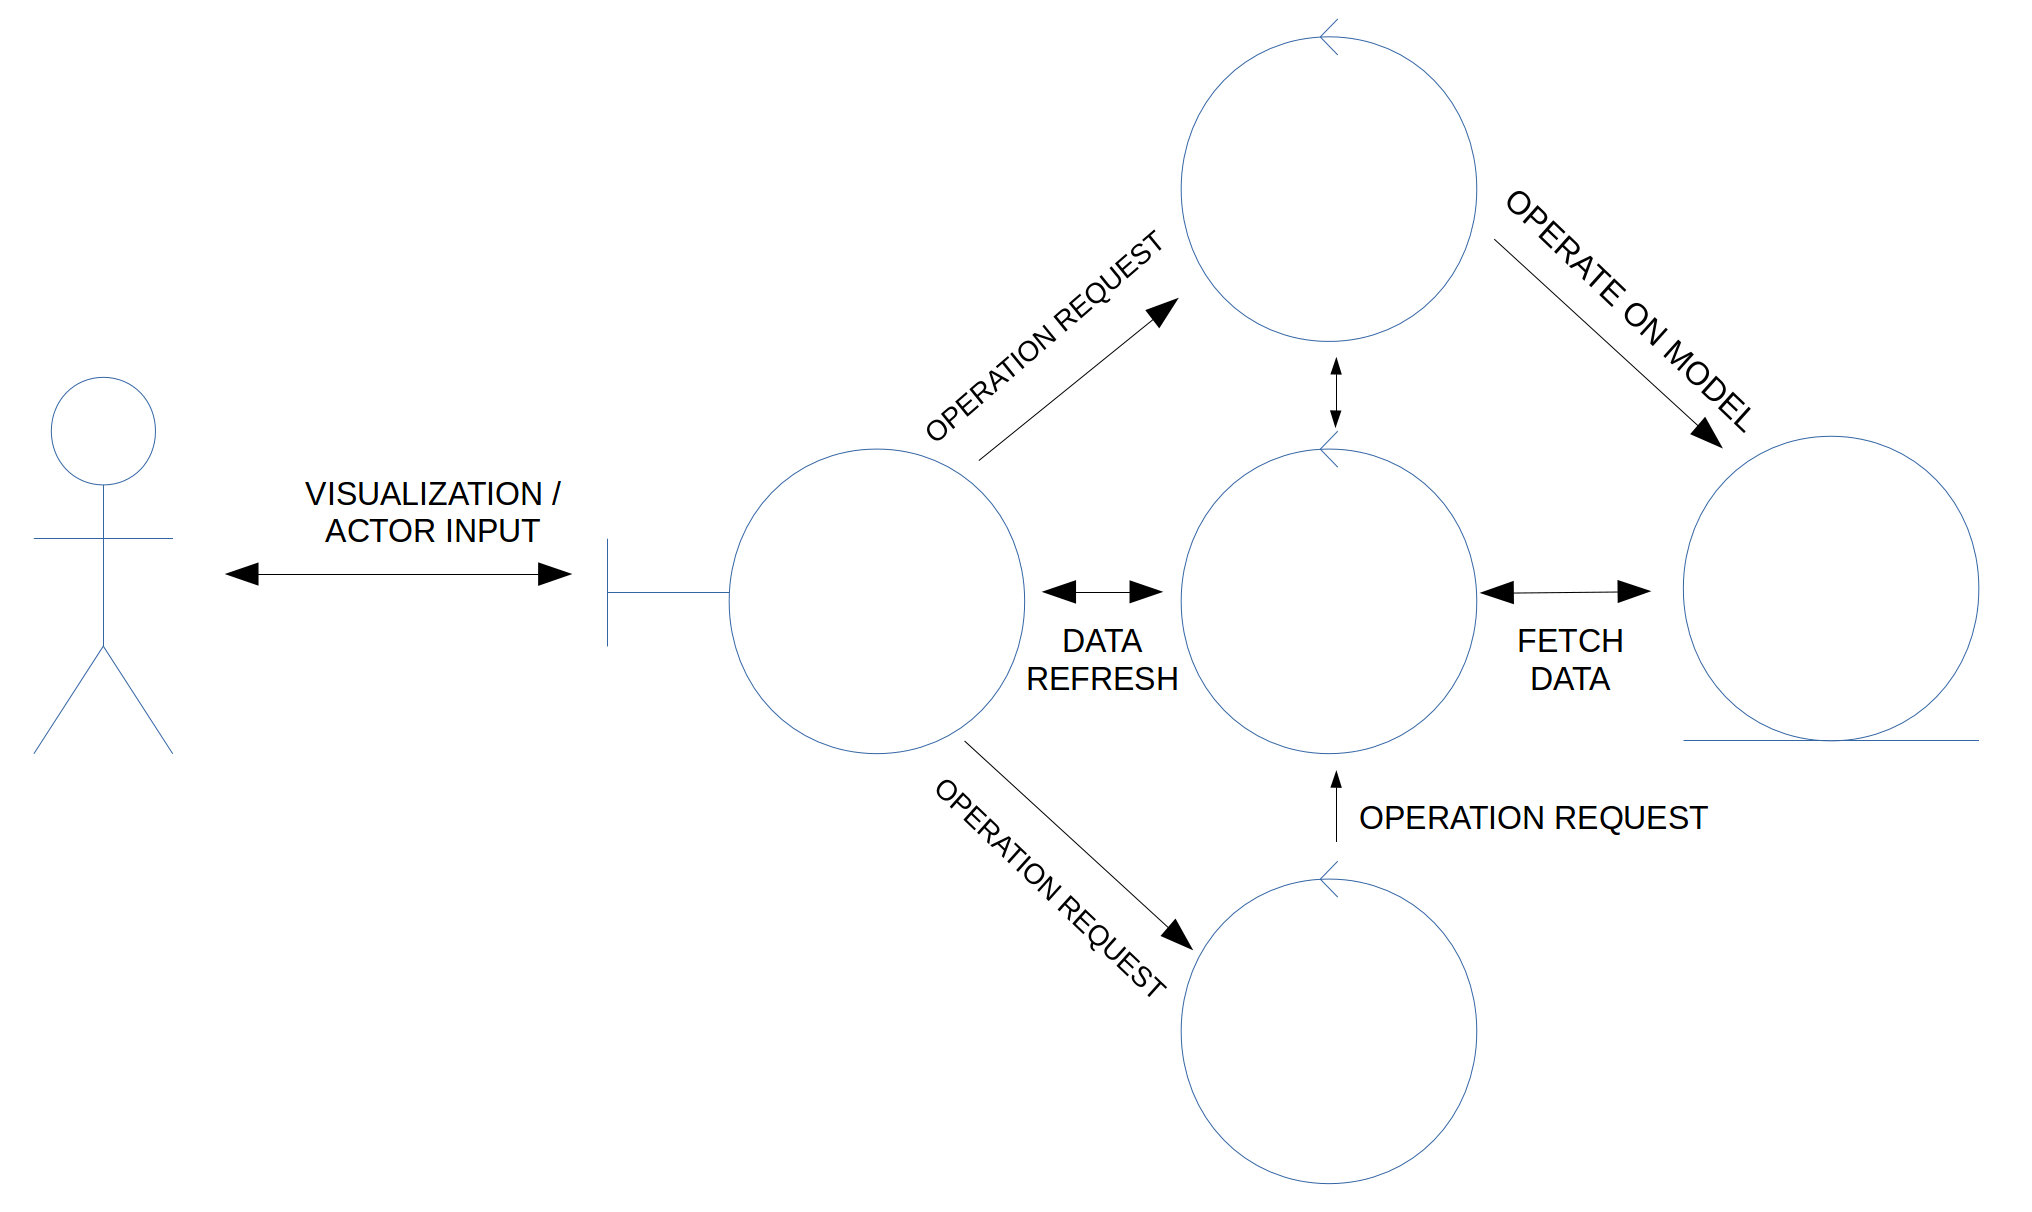
\includegraphics[width=\linewidth]{mvc}
\caption{MVC Architecture UML Diagram}
\end{figure}
In this UML 2.0 (Unified Modeling Language) diagram (robustness analysis diagram, a simplified communication diagram) the 
components are represented as follows (from left to right):
\begin{itemize}
	\item Actor: External agent that uses the system.
	\item Boundary Object: the View component.
	\item Control Objects: the Controller components.
	\item Entity Object: the Model component.
\end{itemize}
This diagram represents how the different components are allowed by the architecture to interact with each other. The View 
can only operate with actors and controllers. Controllers can only operate on the model or other controllers and push data 
to the View. The model can only operate on itself (maintaining the "state" however necessary) and is accessible only to 
controllers. This strict compartmentalization of tasks, allows for very structured applications, that are easy to 
comprehend, maintain and expand upon. Since the actual business logic is contained in controllers, adding logic and 
features to the application becomes as easy as creating a new controller to govern the logic, allocating resources in the 
model to maintain the state, and adding a representation in the view. This breakdown is the true power of the MVC 
architecture, making complex, multi-faceted user interfaces simple to create and expand, while keeping a very simple and 
versatile underlying software structure.\\

HRUI is very well suited to use the MVC pattern. It is essentially a user interface, which requires constant input/output 
to the final user, which is what the MVC pattern was originally envisioned for. But it's also, on the back-end, an 
interface for external robot controllers, and that's where the power of the decoupling between the three components really 
shines in this project. MVC allows for a \textbf{double decoupling} of the application: the separation between how a model 
is represented, and the actual logic that governs the model. In other words, it separates the user experience from the 
programming tasks, both pivoting around the model independently.\\

The user experience is what the View component provides. In this case, the view is an HTML5 web page (which will be 
discussed as a sub-system with an MVC/modular architecture in section \ref{modularfrontendarchitecture}) which grants a 
total decoupling from the host machine, and the back-end as a whole (from this perspective at least, the client-server 
perspective handles that interaction), given this technology's ubiquity. The instructions sent from the View are handled by 
controllers without any knowledge or configuration required by the user. This allows the user to only declare the 
instructions required, without having to process the actual actions. This is the first decoupling.\\

The second decoupling, is that of the model with the actual external robot controllers that need to be programmed for the 
interface to act. The robot programmer or researcher is only aware of the data present in the model at any given time, 
without having to understand anything of how those instructions or data was generated. And most importantly, without having 
to ``care''. For example, the programmer can safely assume that the joystick data present at any time in the model is a 
faithful representation (down to 15 ms accuracy) of the ``state'' of the input. No need to design a user interface, program 
the joystick logic, parse the data through sockets or make an RPC or anything. All the programmer has to do is implement 
his control logic or algorithm, taking inputs and outputs for granted, as they're managed by the integrated controllers. 
This has the enormous advantage of allowing the researcher to do what he's really interested in, programming the robots 
logic, instead of dealing with the work of having to create a user interface.\\

The following diagram, modifies the previous, generic MVC architecture diagram with the particular components of HRUI. It 
does not include all the possible interactions for brevity.\\
\begin{figure}[H]
\caption{HRUI MVC Architecture (see next page)\label{mvcarch}}
\end{figure}
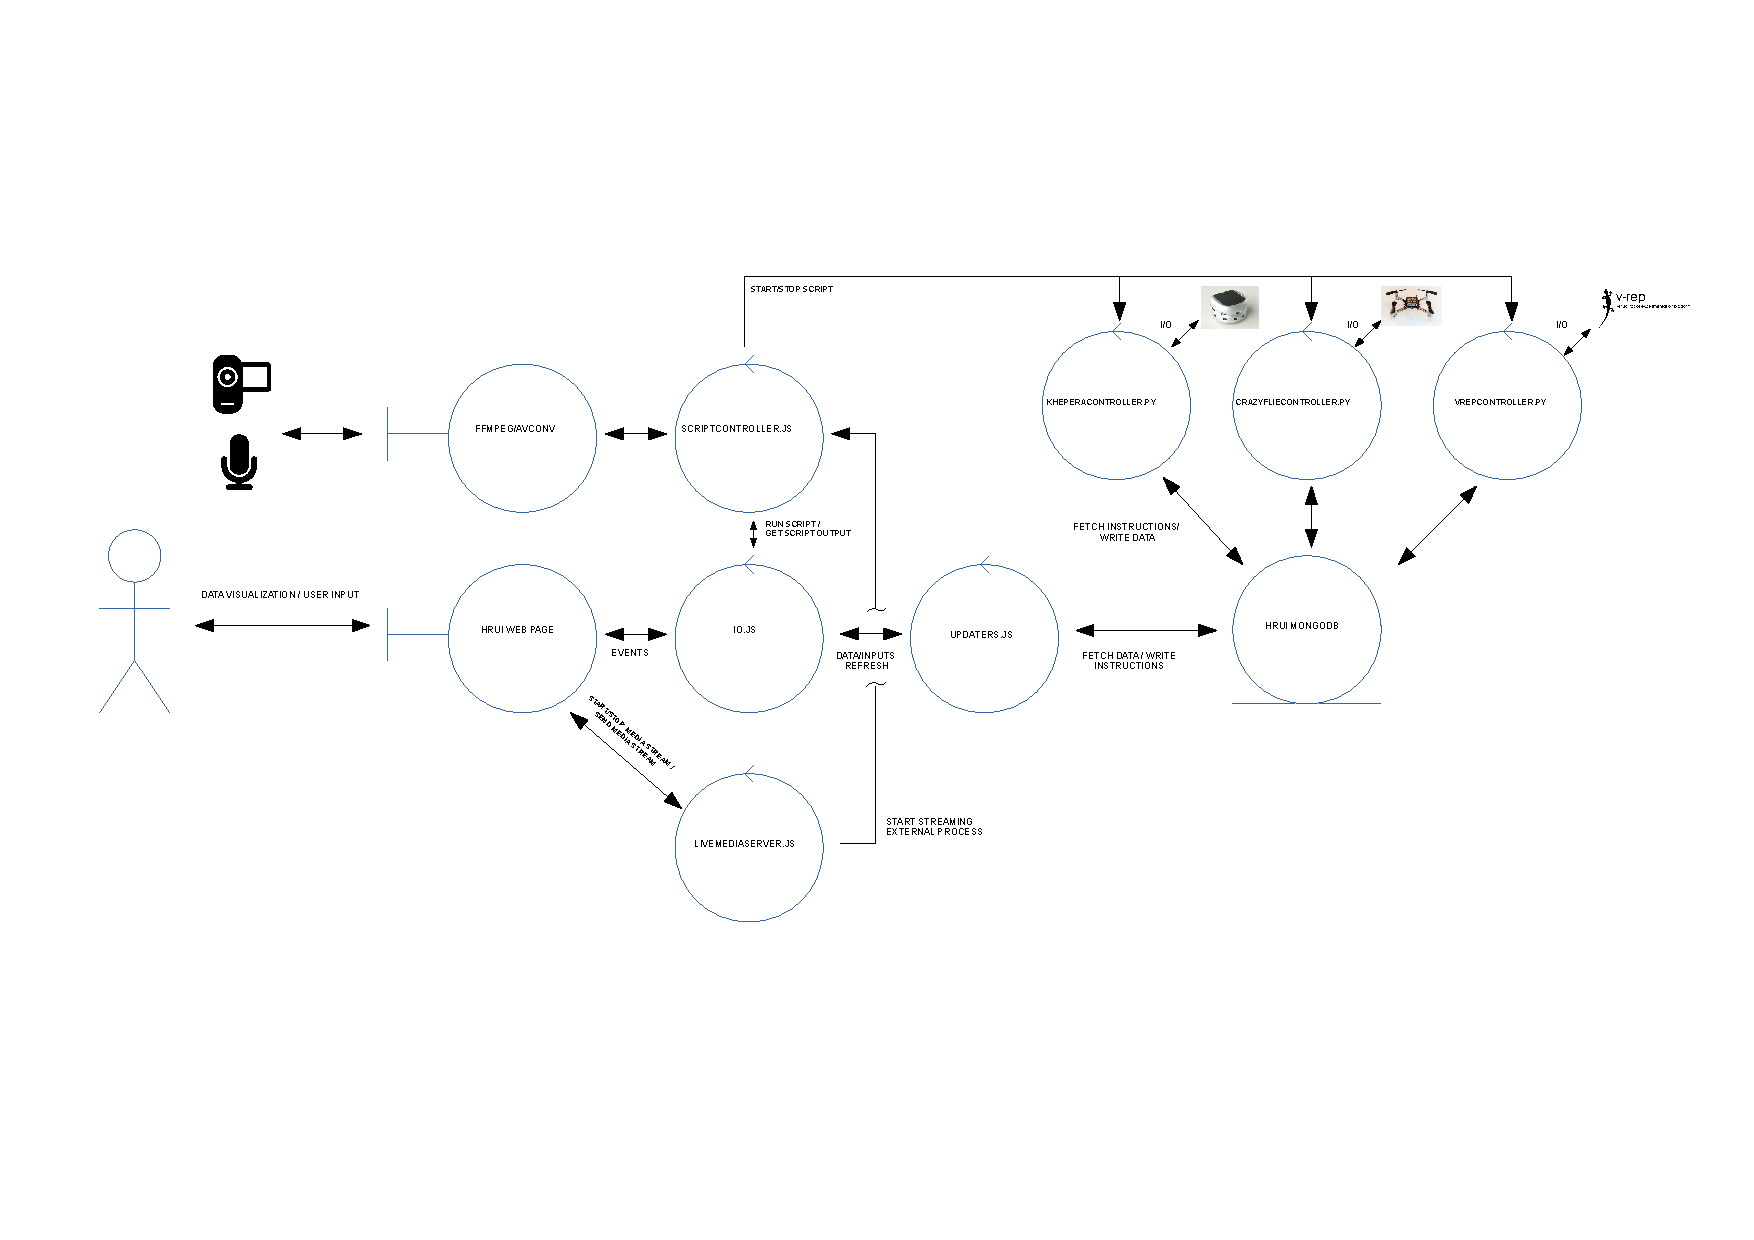
\includepdf[pages={1},landscape]{./img/arch_hrui.pdf}
The following sections briefly describe the structure and functions of each of the components of HRUIs MVC architecture.
\subsection{Model}
The Model component in HRUI is a database that uses the DBMS (DataBase Management System) MongoDB. This technology is 
explained in detail in section \ref{mongodb}, but the main gist is that it's a NoSQL database, making it particularly 
suitable for real-time system r/w requirements and it stores data as documents, which are simply JSON (JavaScript Object 
Notation) formatted objects. In the system architecture, represented in figure \ref{mvcarch}, the Model is the Entity 
object, and can only be accessed directly by control objects, isolating it from the View.\\

HRUIs database has only one collection of documents, called data, in which the state of the application is maintained. It 
initially includes 10 documents, or items, but can be expanded as much as necessary depending on the requirements of each 
robot. Each item must have two properties, for identification purposes:
\begin{itemize}
	\item ``\_id'': An integer value used to identify the item, unequivocally. 0-9 are reserved for the default items.
	\item ``item'': A string that indicates the item's contents.
\end{itemize}
The initial 10 items are:
\begin{itemize}
	\item joystick: holds the state of the primary joystick.
	\item robotData: holds the location, speed, orientation and angular speed of the robot.
	\item robotGeolocation: holds the robots latitude and longitude, and the accuracy in meters.
	\item customDataTest: holds dummy data to test custom data module.
	\item profiles: holds the saved profiles for the profile management module.
	\item mapData: holds a 300x300 binary matrix (0 equals blank, 1 equals obstacle) as a model of the map shown in the 
	data monitor module, which can be used to create a SLAM system.
	\item deviceData: holds the orientation and motion data of the client device.
	\item joystick2: holds the state of the secondary joystick.
	\item voiceCommand: holds the last command registered in the voice command module.
	\item gamepad: holds the state of the gamepad, as registered by the gamepad module.
\end{itemize}
These items hold the basic data required by some of the application modules to function, but the model is in no way limited 
to these items. The programmer can add as many items of any level of complexity as required, for use in different 
controllers or to output to the view through the custom data module, if need be. The same works in the opposite direction, 
the user can add as many inputs as necessary from the View, on the fly, using the custom input module, that can be 
retrieved just as any other item from a controller. This showcases once again the benefits of the MVC pattern, and in the 
case of HRUI the double decoupling of the user interface from the model and likewise with controllers.
\subsection{View}
The View in HRUI is of course the HTML5 web page. The view is considered a sub-system, and has its own architecture, 
described in section \ref{modularfrontendarchitecture}. In the overall MVC architecture, represented in figure \ref{mvcarch}
, the View is the main boundary object, and the only way an actor (in this case the user) can interact with the system, 
thus isolating the actor from the actual procedural logic, and from the model.\\

As each individual module will be discussed in section \ref{modularfrontendarchitecture}, this section only briefly 
explains the overall layout of the UI.\\

The web page, in it's standard format, used in wide screen devices (i.e. Desktops/ Laptops/ Tablets), uses a three column 
layout to present the modules to the user, organized as follows:
\begin{itemize}
	\item \textbf{Left Column. Inputs}: 4 Modules: Primary Joystick, Custom Inputs, Device Orientation and Voice Commands.
	\item \textbf{Center Column. Multimedia}: 3 Modules: Live Video, Live Audio and Geolocation Map.
	\item \textbf{Right Column. Outputs/Utilities}: 4 Modules: Data Monitor, Custom Data, Script Execution (Secondary 
	Joystick is placed here for ergonomic reasons). 
\end{itemize}
This maximizes access to controls when using a multi-touch landscape device, like a tablet, by keeping controls on the 
sides of the page, and the live video stream in the center. The layout is liquid, which means it automatically tries to 
adapt to the viewport (the section of the browser where the page is rendered) and its dimensions dynamically. If the window 
is resized, the layout tries its best to place all different modules in the most readable way, limited obviously by the 
minimum usable size.\\

Using CSS3 media queries (see section \ref{html5styling} for more), the layout changes to a one column design when the page 
is used on a smartphone, or otherwise portrait oriented device. Since it's not possible to represent even a few modules at 
the same time on a small, vertical screen, the layout maximizes the use of one module at a time, allowing the user to 
scroll from one to the other as needed. It also frees up screen real estate by hiding the module selection toolbar in a 
side menu, that can be pulled out and hidden by using the menu button at the top left of the page. This toolbar can also be 
hidden in the desktop version.
\begin{figure}[H]
\centering
\subfloat{{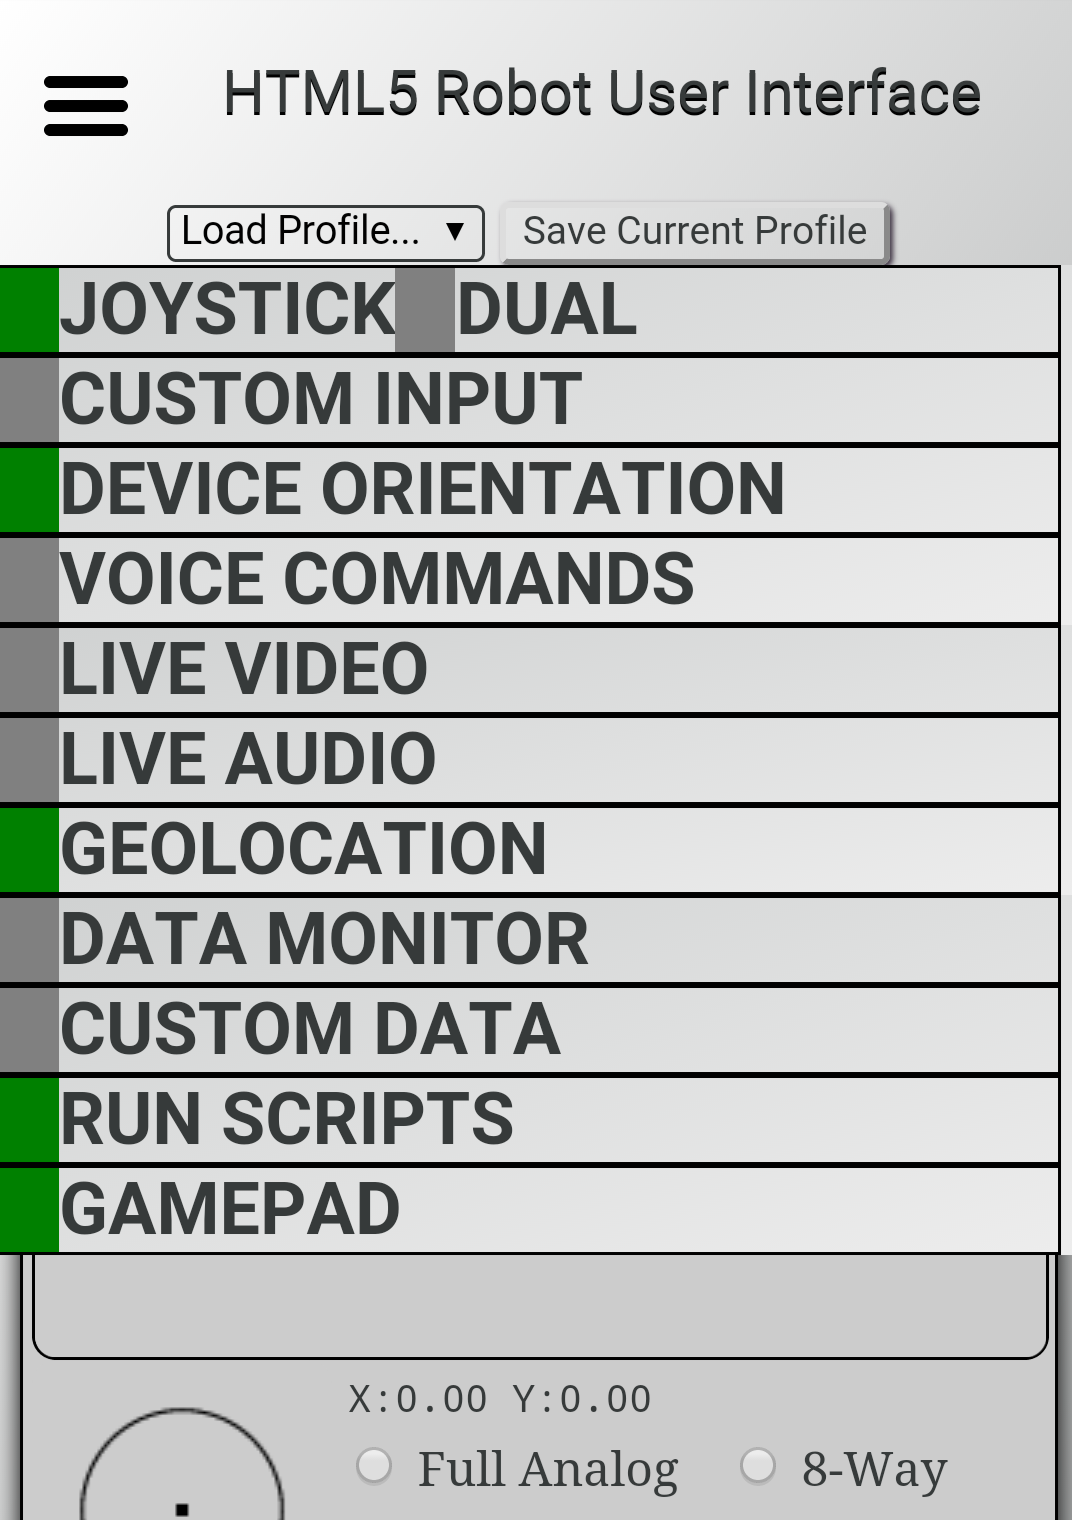
\includegraphics[width=\linewidth/5]{sidebar}}}
\subfloat{{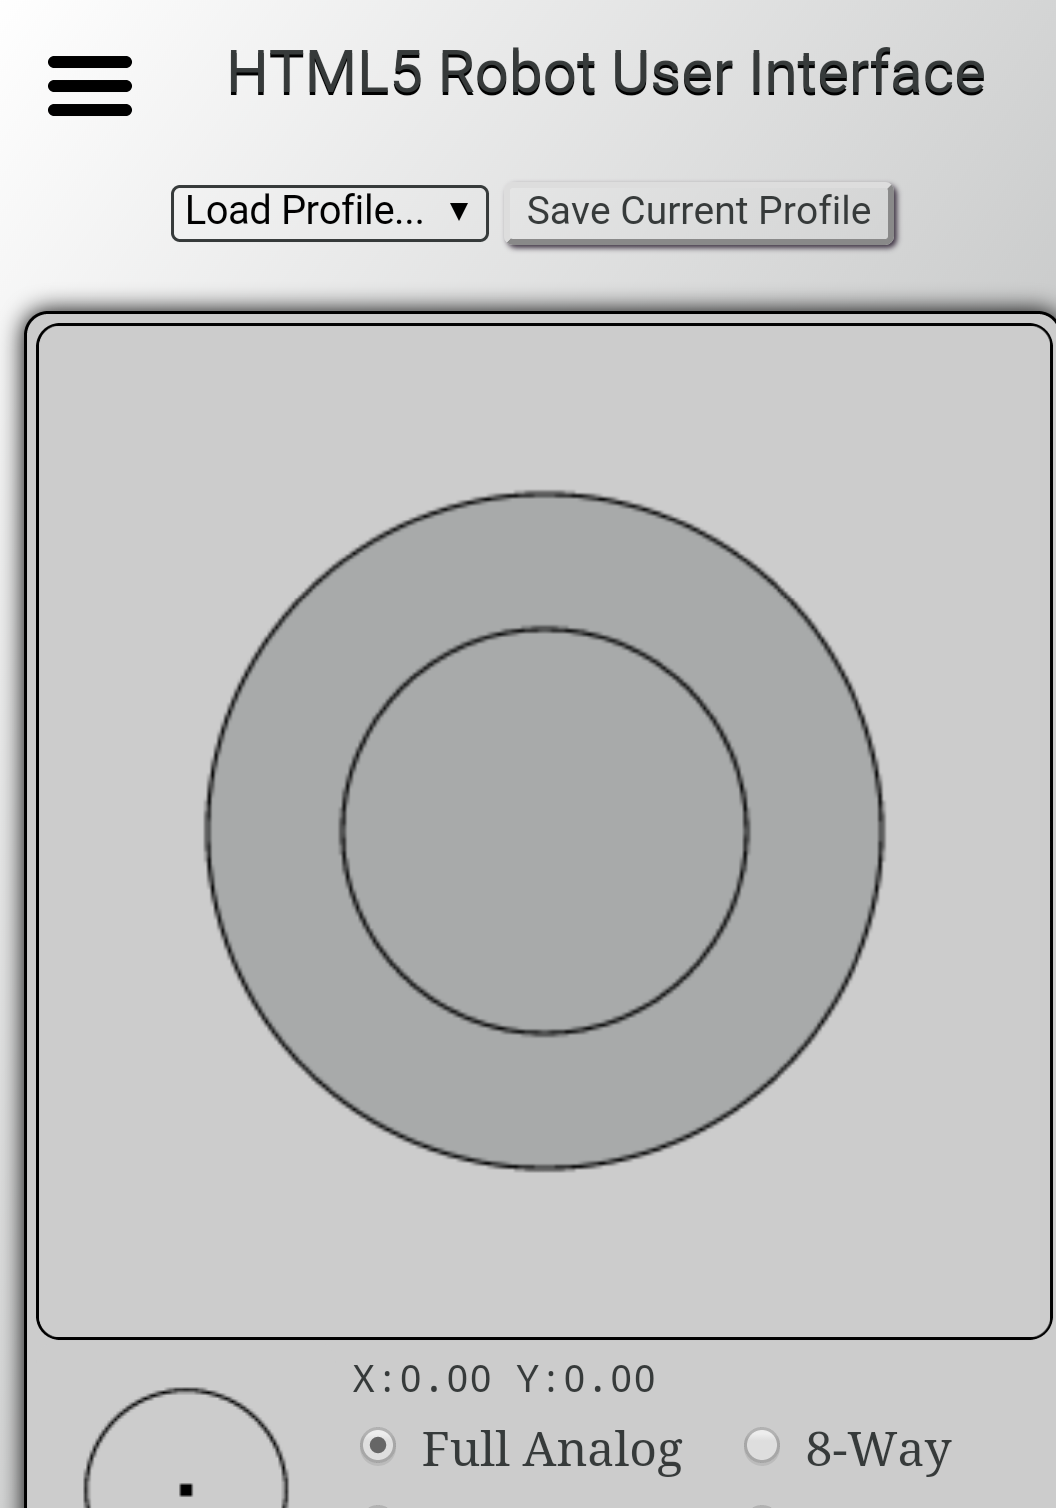
\includegraphics[width=\linewidth/5]{nosidebar}}}
\caption{HRUI Mobile Side Bar}
\end{figure}
\begin{figure}[H]
\centering
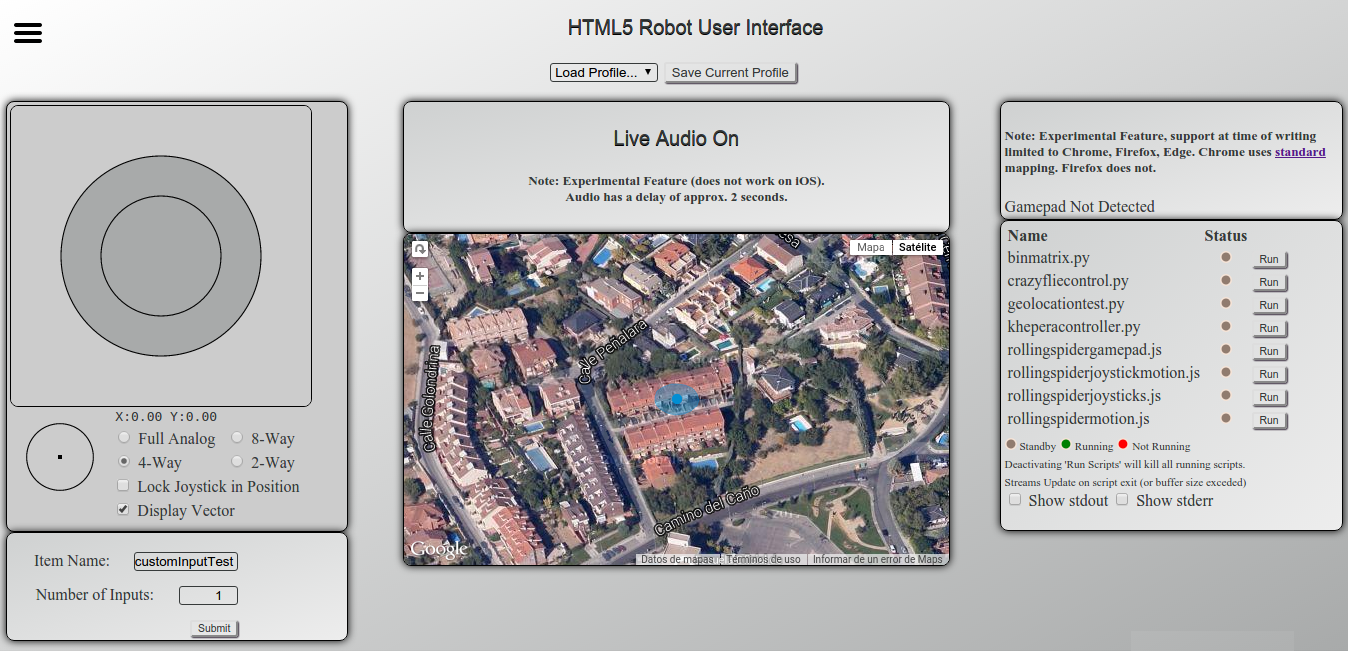
\includegraphics[width=\linewidth]{hrui3column}
\caption{HRUI Desktop/Laptop/Table Three column design (Toolbar hidden)}
\end{figure}
\subsection{Controllers}
HRUI controllers are divided in two distinct categories:
\begin{itemize}
	\item \textbf{Internal Controllers}: They're integrated in the application, controlling the inputs and outputs from the 
	view to the model. In the system architecture (figure \ref{mvcarch}), they are represented between the View and the 
	Model. There are four main internal controller modules: updaters.js, scriptController.js, io.js and liveMediaServer.js.
	\item \textbf{External Controllers}: Designed by the programmer or researcher to input and output data between the 
	model and a robot/s. In the system architecture (figure \ref{mvcarch}), they're represented between the model and the 
	robots. They're not integrated in the application and can only interface with the model and their respective robots 
	directly. As a proof of concept, three external controllers have been developed to control three different robots, all 
	three written in the Python programming language (see section \ref{python}): 
	\begin{itemize}
		\item vrepcontroller.py: controls a virtual Khepera III robot in the robot simulator V-REP (see section 
		\ref{vrepvirtualkheperaiii}).
		\item kheperacontroller.py: controls a Khepera III robot (see section \ref{kheperaIII}).
		\item crazyfliecontroller.py: controls a Crazyflie 2.0 drone (see section \ref{crazyflie2}).
	\end{itemize}
\end{itemize}
\subsubsection{Internal Controllers}
\begin{itemize}
	\item \textbf{updaters.js}: This module is the controller that collects all requests from other controllers to modify 
	or get data in the model and processes them. It's represented in the system architecture (figure \ref{mvcarch}) between 
	io.js and the model. Each of the functions it holds can be considered itself a sub-controller, that is designed to 
	respond to each distinct requests. The power of the MVC architecture allows this code to be reasonably close the 
	business logic, making it easily comprehensible and maintainable. The module exposes an interface to other modules, to 
	call the necessary update to the database as needed. The main consumer of this interface is io.js.	
	\item \textbf{io.js}: Configures the Socket.IO framework (see section \ref{html5websockets}) to capture and send events 
	to and from the View. It's represented in the system architecture between the View and the rest of the controllers (
	except for liveMediaServer.js, that interacts directly with the view for media streaming). The event model will be 
	discussed in section \ref{clientserverpattern} as part of the Client-Server pattern. After initial configuration, this 
	module simply declares ``hooks'' for each event. This means it establishes a handler function (a controller in itself) 
	to process each event. The handler functions are exposed by updaters.js and scriptController.js, to service the request 
	of the View, or other controllers.
	\item \textbf{scriptController.js}: Handles requests from other controllers and from the view to execute or kill 
	external scripts and programs. This includes starting and ending avconv/ffmpeg media stream acquisition and running and 
	killing JavaScript and Python scripts added to the userscripts folder (normally, these will be external controllers, 
	but not necessarily) at the request of the View (through an io.js event hook). Requests to this controller are made by 
	io.js and liveMediaServer.js.
	\item \textbf{liveMediaServer.js}: Configures media stream reception and relay to the View, using raw websockets (see 
	section \ref{html5websockets}).
\end{itemize}
A UML 2.0 Communication/Collaboration diagram for internal controllers is presented in figure \ref{controllerarch}. 3 Use 
cases are presented in the diagram:
\begin{enumerate}
	\item User moves virtual joystick. Triggered by the user through a mouse/touch event.
	\item Periodic update of robot data (position, orientation, velocity and angular velocity).
	\item User turns on Live Video feed.
\end{enumerate}
This diagram uses the following format to represent messages between objects:\\

\centerline{[sequenceNumber.] methodName(parameters) [: returnValue]}
\begin{itemize}
	\item {[}sequenceNumber.{]} : Numbering that indicates the order of messages for each use case.
	\item methodName(parameters) : The ``method'' invoked and the parameters passed. Method is used in the sense of object 
	oriented programming, where any action that an object requests from another is called a method. Parameters are 
	arguments that the invoked action requires.
	\item {[}: returnValue{]} : The response data received after the invocation of the method, if any.
\end{itemize}
\subsubsection{External Controllers}
Since the external controllers depend on how each robot's API is implemented, it's particular inputs and outputs and 
communication method, the UML 2.0 communication diagram presented in figure \ref{extcontrollerarch} is very abstract, 
devolving into a component diagram between the robot and the controller indicating the interface exposed by the robot and 
it's required implementation.
\begin{figure}[H]
\caption{HRUI Internal Controllers Communication Diagram (see next page)\label{controllerarch}}
\end{figure}
\begin{figure}[H]
\caption{HRUI External Controllers Communication Diagram (see next page)\label{extcontrollerarch}}
\end{figure}
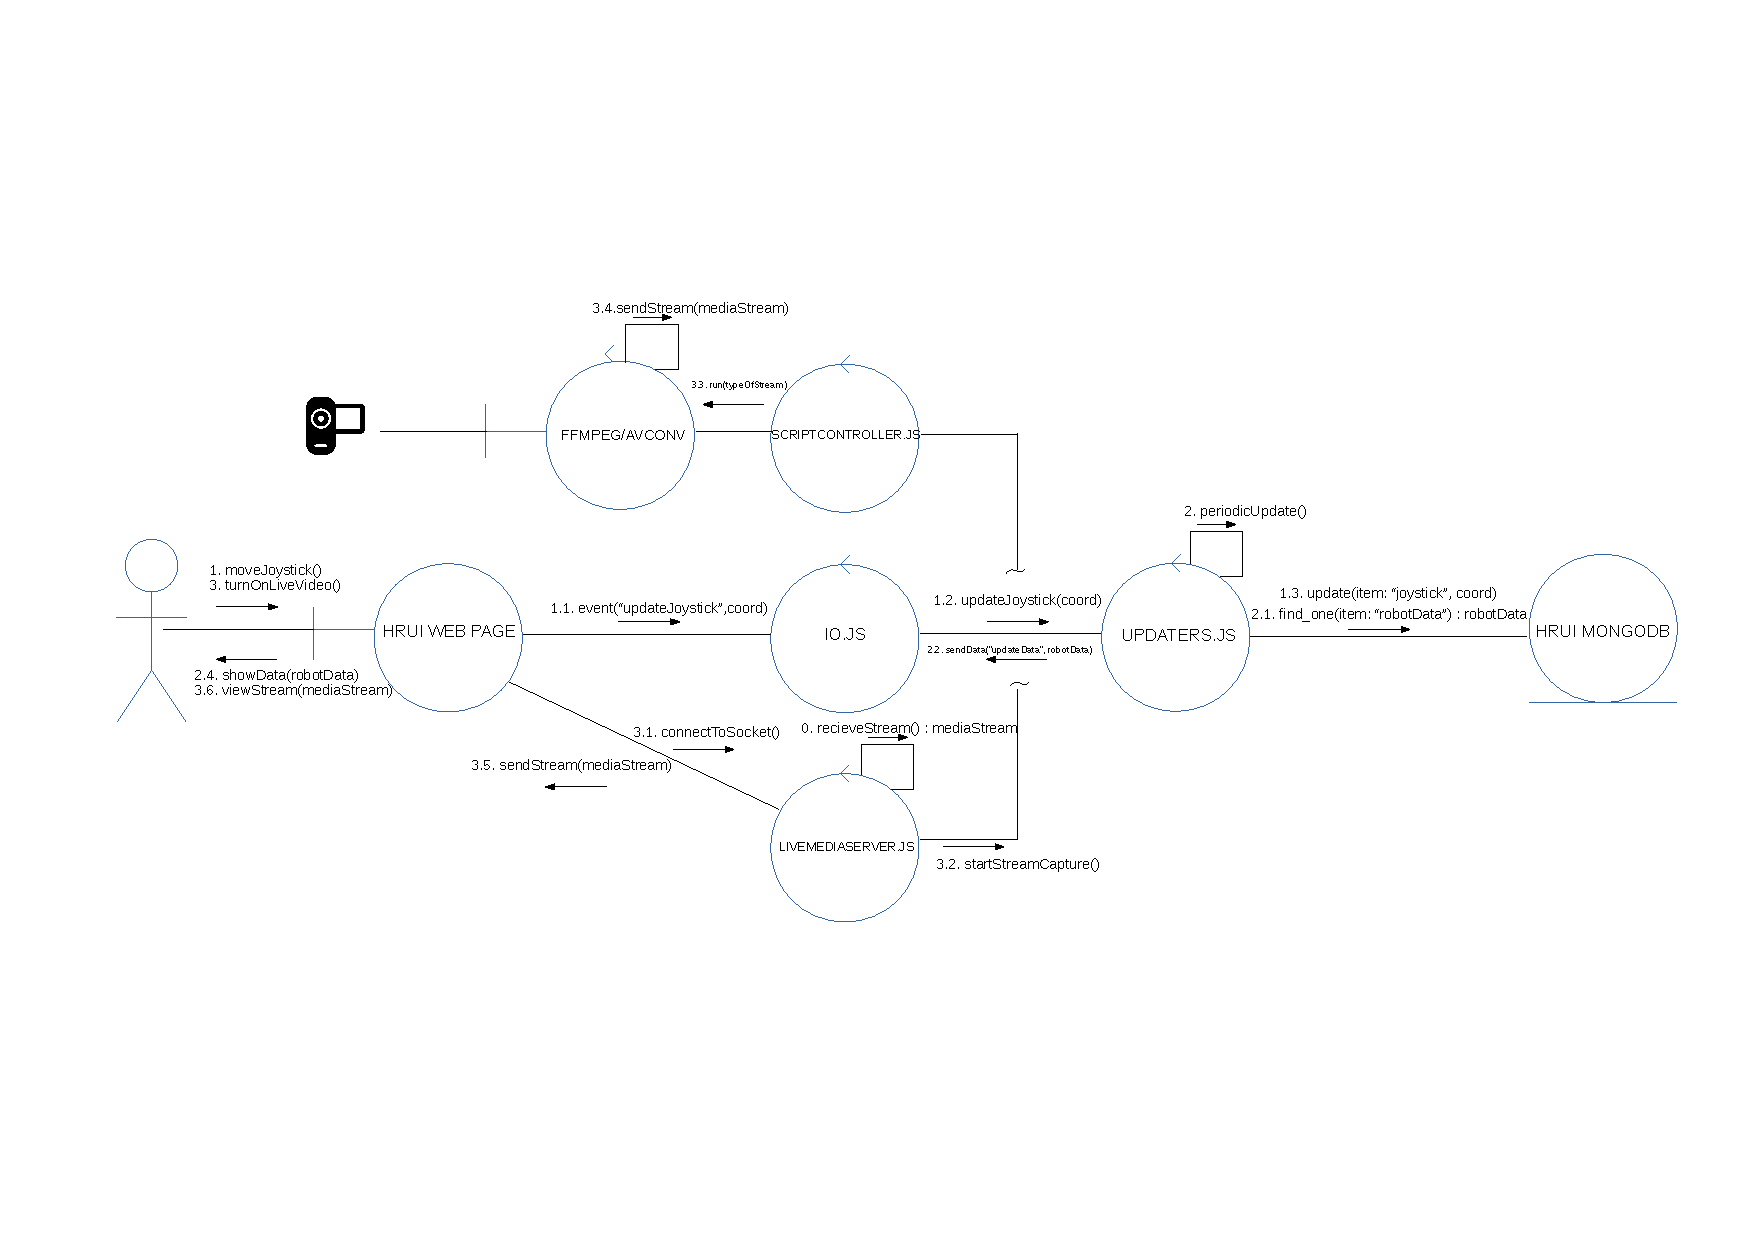
\includepdf[pages={1},landscape]{./img/arch_controllers.pdf}
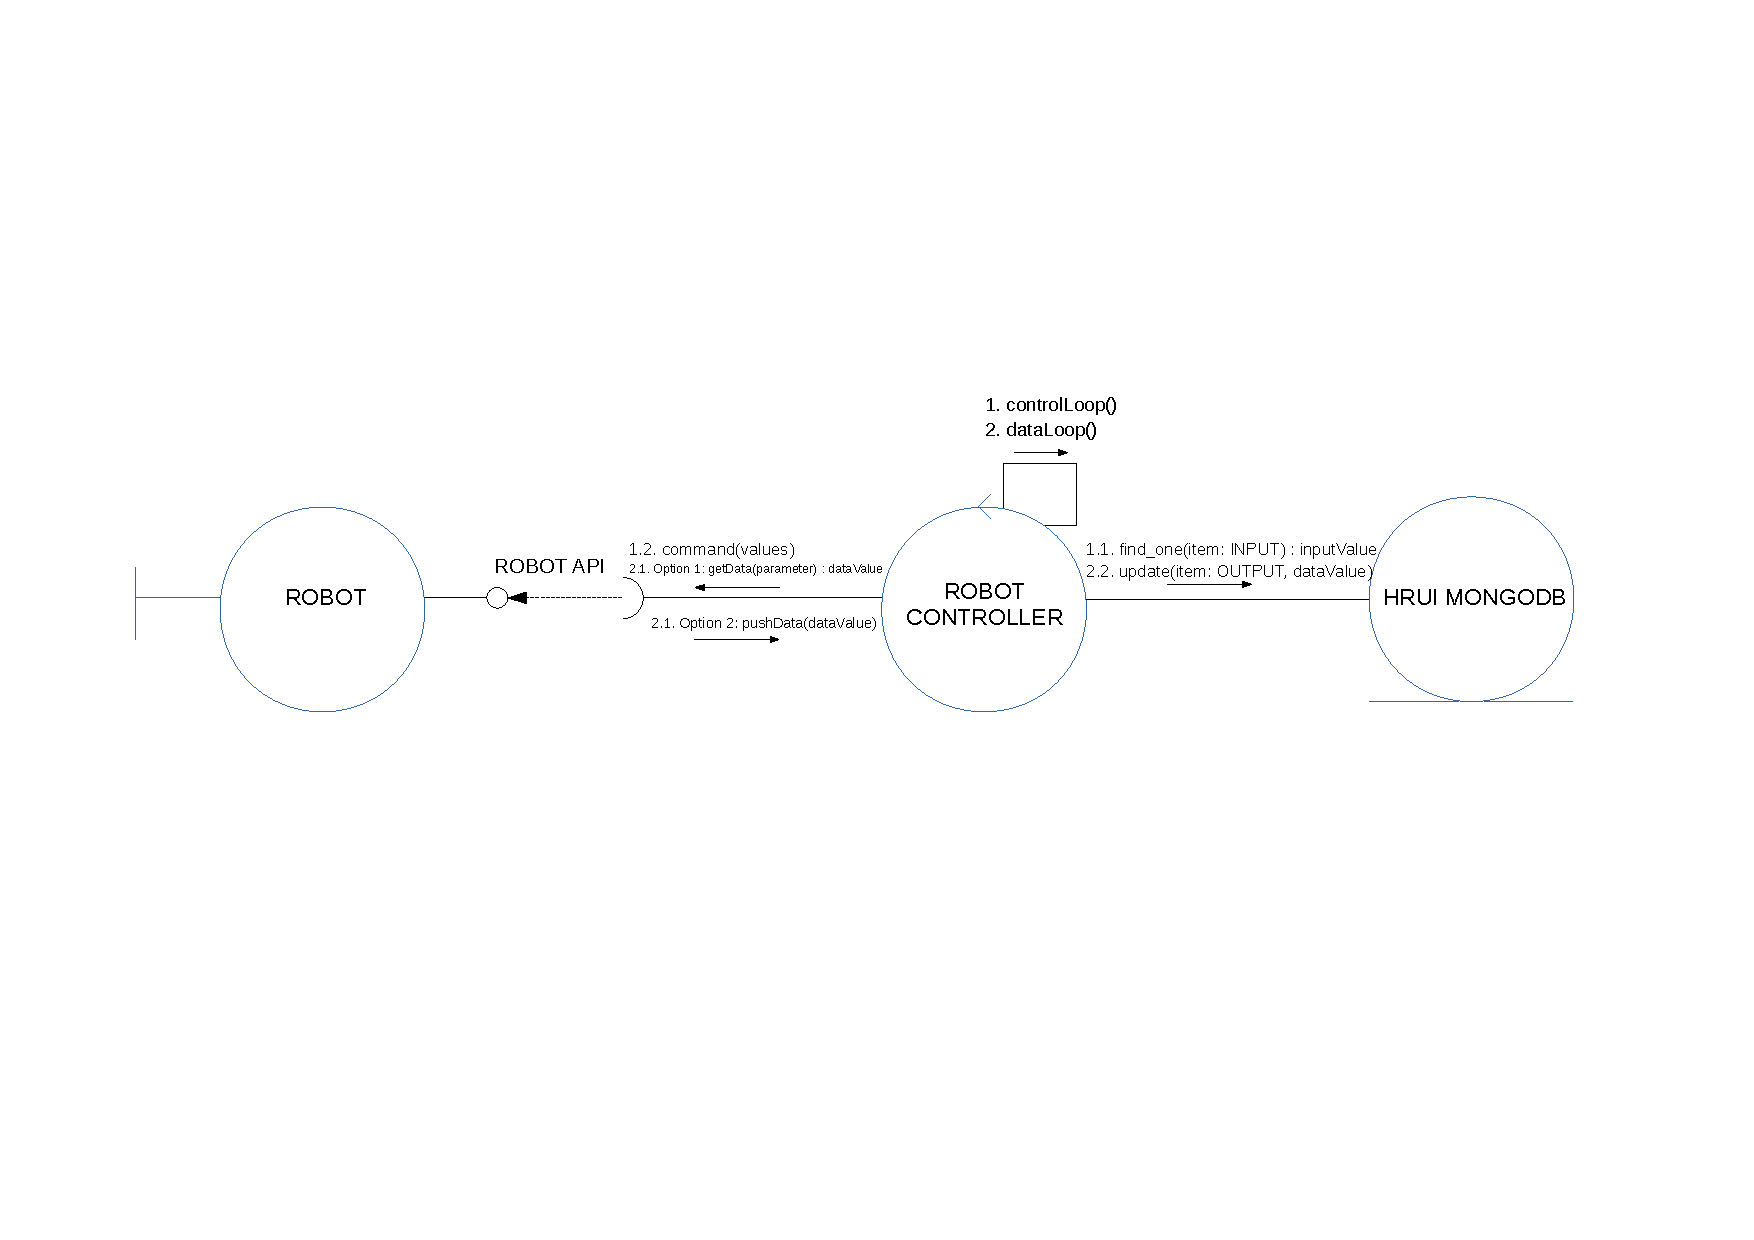
\includepdf[pages={1},landscape]{./img/arch_ext_controllers.pdf}
\section{Client-Server Pattern} \label{clientserverpattern}
The Client Server Pattern is a structure for distributed software (software that is run on different machines pertaining to 
the same system or in order to achieve a common goal or service) that separates components into two main stereotypes:
\begin{itemize}
	\item \textbf{Client}: A component that requests services and resources from a server, and does not provide any of it's 
	own resources to other components. Generally there are multiple clients per application, although this is not a 
	requirement.
	\item \textbf{Server}: A component whose purpose is to provide services and resources to clients. Typically there is only 
	one server component, although this server itself can be a distributed system across many machines that relate to each 
	other using the same client-server pattern.
\end{itemize}
The components communicate with each other using requests and responses, which are simply messages between components, that 
are encoded in a pre-shared protocol readable by both machines. The most evident example of the Client-Server model is the 
World Wide Web, and the protocol that underlies beneath it, HTTP. This technology is covered more in depth in section \ref{HTTP}, including a full message exchange between client and server, but the main gist is that a client always initiates the 
communication by issuing a request to the server; the server receives the request and processes it in any way necessary; 
finally, the server returns a response to the client, returning to the same state as before the connection was established. 
This last part is important, as it's typical for a Client-Server model to have a \textbf{stateless} server. This means that 
the server has no "memory", nor does it hold any static data that survives a client transaction. In other words it doesn't 
hold a ``model'' or "state". This is not an issue or problem with the pattern, it's actually one of its biggest strength. By 
not keeping a state, the interactions between client and server stay very simple and very close to the business logic. As with 
all software patterns, the client-server architecture is designed to compartmentalize code, structure it, so that it's easier 
to comprehend and in consequence easier to develop and maintain. However, as with all patterns, it's not a standalone solution 
to any system. Patterns solve a particular scenario, in this case communication between components. For some systems, this 
solution is complete. Most notably, the whole World Wide Web basically functions using only this paradigm. But as the web has 
evolved (see sections \ref{HTTP} and \ref{HTML} for a brief history on the webs evolution), resources have ceased to be static 
documents, and services have become real-time applications. The client-server paradigm is not designed to handle this, and 
therefore is an incomplete solution to web applications, mainly because of it's primary advantage: statelessness. Applications 
of a certain level of complexity, require a model, that holds all the data that makes the state of the application evolve. 
This is why most web applications have integrated into the client-server distributed solution, another architectural pattern: 
the Model View Controller pattern. HRUI is one such application, and the MVC architecture perspective is discussed in depth 
the previous section, \ref{mvcpattern}.\\

HRUI as a distributed application, requires a communication structure for it's components, and it uses the client server 
paradigm to achieve this structure, with three key deviations from the typical client-server pattern:
\begin{itemize}
	\item \textbf{\textit{Stateful} Server}: (\textit{Stateful}: a made up word by the computer science industry, meaning the 
	opposite of stateless). The inherent nature of HRUI as an application means the server cannot be stateless, as no 
	significant input/output can occur if the current state is not being held in a model.
	\item \textbf{Event driven Communication}: Instead of using a request/response communication protocol, like HTTP, the 
	communication is made by events (messages that carry a data package attached to it) which are generated by the client as 
	well as the server. Which leads to the third deviation.
	\item \textbf{Data push from server}: As a consequence of the event driven communication protocol, the Client does not 
	always initiate a transaction through a request and receives a response from the server. In some events data is "pushed" 
	to the client from the server, without the client requesting it previously.
\end{itemize}
It might seem as though these deviations are breaking the pattern, but this is not entirely the case. The pattern doesn't 
imply statelessness nor does it prohibit data pushing. These are just typical implementations of the paradigm. The pattern 
only implies that a server provides its resources to a client that doesn't share its own. It can be fairly argued that event-
driven communication is an architecture pattern in itself, but the fact is, it's just the protocol that communicates the 
processes. The actual purpose of the processes is what should define the architecture, and in this case, one process strictly 
serves the other. The server never requests resources from the client, and the client unloads much of the heavy lifting onto 
the server, leveraging it's resources. This is a clear case of client-server structure.
\subsection{Server}
The server is a JavaScript program that is built on the node.js platform. This technology is discussed in depth in section 
\ref{nodejs}, but the main gist is that it's a non-blocking, event-driven framework, designed for distributed applications and 
scalability. The most important part of this is that it's a non-blocking runtime, meaning that processing is done 
asynchronously, which makes for a very efficient server, especially for responsive web applications. Since nothing has to be 
processed immediately after a request is made, the server can delegate to the CPU scheduler what process has a priority at any 
time, allowing more intensive processing to finish quicker, not interrupted by less demanding requests that will generally 
take next to nothing to process.\\ 

Another advantage of node.js is that the server can be deployed on basically any general purpose operating system available, 
given that the platform is available for all of them. This made possible the development of a portable server using a 
Raspberry Pi 2 running Arch Linux (see section \ref{raspberrypi2} for more).\\

The server uses two protocols two communicate with clients: HTTP and WebSockets. The former uses an Express framework server, 
to serve the static content of the web page using the HTTP Protocol, discussed in section \ref{HTTP}. The structure of an 
Express server is discussed in section \ref{express}, with examples of how it's used in HRUI. The latter is used in two 
distinct ways: using an event-driven communication protocol, (discussed in section \ref{eventdrivencommunicationprotocol}), 
and using raw websockets. The first is used for the general exchange of inputs and outputs between server and client, while 
the second is used for media streaming.\\

Media Streaming is handled by the module liveMediaServer.js on the server side. On activation by the user of one of the two 
live streaming modules (Live Video and Live Audio), a WebSocket connection is established from the client, to the server, that 
is permanently listening for connections. On connection, liveMediaServer.js requests external programs to start media 
acquisition through another module (represented in MVC controller architecture use case 3, figure \ref{controllerarch}). Once 
acquisition has begun, liveMediaServer.js relays the bit stream from the external programs to the client, where it's decoded 
(see sections \ref{livevideo} and \ref{liveaudio} for more on how this is done).
\subsection{Client}
The client is the HTML5 web page. The internal architecture of the client is discussed as a subsystem in the following 
section, \ref{modularfrontendarchitecture}. From the client-server perspective, the client initiates the communication 
protocol using the HTTP protocol (see section \ref{HTTP}), and requests the static resources that are included in the HTML 
(see section \ref{HTML}). Once the resources are collected, the client runs the requested scripts, that upgrade the HTTP 
connection into a WebSocket connection (see section \ref{html5websockets}), through the Socket.IO framework, enabling the event
-driven communication protocol, that effectively replaces the HTTP request-response protocol for the remainder of the session.
\subsection{Event-Driven Communication Protocol} \label{eventdrivencommunicationprotocol}
The event-driven communication protocol used in HRUI is powered by Socket.IO, a JavaScript framework. The framework is built 
upon the technology of HTML5 WebSockets, discussed in section \ref{html5websockets}, where an example of an event-driven 
transaction is shown. This communication protocol is essential to building a real-time web application that is responsive and 
fast. A WebSocket is a bi-directional (``full-duplex'') communication channel established between the client and the server 
(see section \ref{html5websockets} for a more detailed explanation). What Socket.IO does is abstract this communication 
channel into an interface where each component can send and receive messages with a data package attached to it, at any given 
point at run time. Both the client and the server have handler functions attached to each event type, that process the data 
package in whatever way necessary.\\

In HRUI, the Server holds all the handler function registration in one module: io.js (see the previous section \ref{mvcpattern}
, where this module is described as a controller in the MVC architecture). This module sets up the Socket.IO WebSocket to 
listen for incoming connections, and on receiving a new connection, registers callbacks (handler functions in JavaScript 
jargon) for all required events.\\

The actual processing is done in different modules. In the example shown in figure \ref{iojs}, the module updaters.js handles 
the request from the client to store a new value for the joystick in the model (Use Case 1, as presented in figure 
\ref{controllerarch} from the MVC Architecture perspective). This separation is intentional, to keep the communication logic 
separate from the actual business logic, improving maintainability, readability and scalability of the code.\\
\begin{figure}[H]
\centering
\captionsetup{justification=centering}
\RecustomVerbatimEnvironment{Verbatim}{BVerbatim}{}
\begin{minted}[fontsize=\footnotesize]{javascript}
function(io) {
    io.on('connection', function(newsocket) {
        socket = newsocket;
        // log user connect
        console.log('HRUI IO: A User Connected.');

        // log user disconnect
        socket.on('disconnect', function() {
            console.log('HRUI IO: A User Disconnected.');
        });
        // receive joystick position
        socket.on('updateJoystick', function(data) {
            updaters.updateJoystick(data);
        });
        /* 
        	All other event handlers removed for clarity,
        	as they have the same structure as `updateJoystick'
        */
    });
};
\end{minted}
\caption{HRUI io.js Event Callback Configuration (heavily abridged for clarity)\label{iojs}}
\end{figure}

A UML Sequence Diagram is presented in figure \ref{clientserverarch} for the Client-Server pattern. It represents a timeline 
for an HRUI session, with all the communication transactions that take place between client and server. Only two processes are 
represented, even though many other components provoke the interactions that take place, to focus exclusively on the 
communication between client and server, given that the other interactions are well represented in other architecture diagrams 
(figures \ref{mvcarch} and \ref{controllerarch}). The dashed lines represent the lifelines of the processes, in other words 
the life span of the process. The blocks on top of the lifelines are activation boxes, that signify processing information. 
The arrowed lines between lifelines represent messages between processes, with the arrow indicating the direction of 
communication. It should be noted that event-driven communication isn't represented with activation boxes to emphasize the 
difference between processing that is done by the server component (represented with activation boxes) and processing done by 
other components (represented without activation boxes). Event-driven communication obviously results in processing, but this 
workload is offloaded to other components, that handle the business logic attached to the message, not the communication 
logic, as explained earlier.\\

As a side note, it's interesting to point out that the model of the application has it's own client-server architecture. 
MongoDB is a distributed DBMS (DataBase Management System), meaning that access to the model is in no way tied to the server. 
In fact, the model can be accessed on a network, so robot controllers can be run on completely different machines than the 
server. This means that the application could even work with the user accessing the server through the Internet, and the 
server being accessed by the controller through another Internet connection. A server in one part of the world could be 
receiving inputs from another part of the world, and those inputs being applied to a robot in a third international 
destination.
\begin{figure}[H]
\centering
\captionsetup{justification=centering}
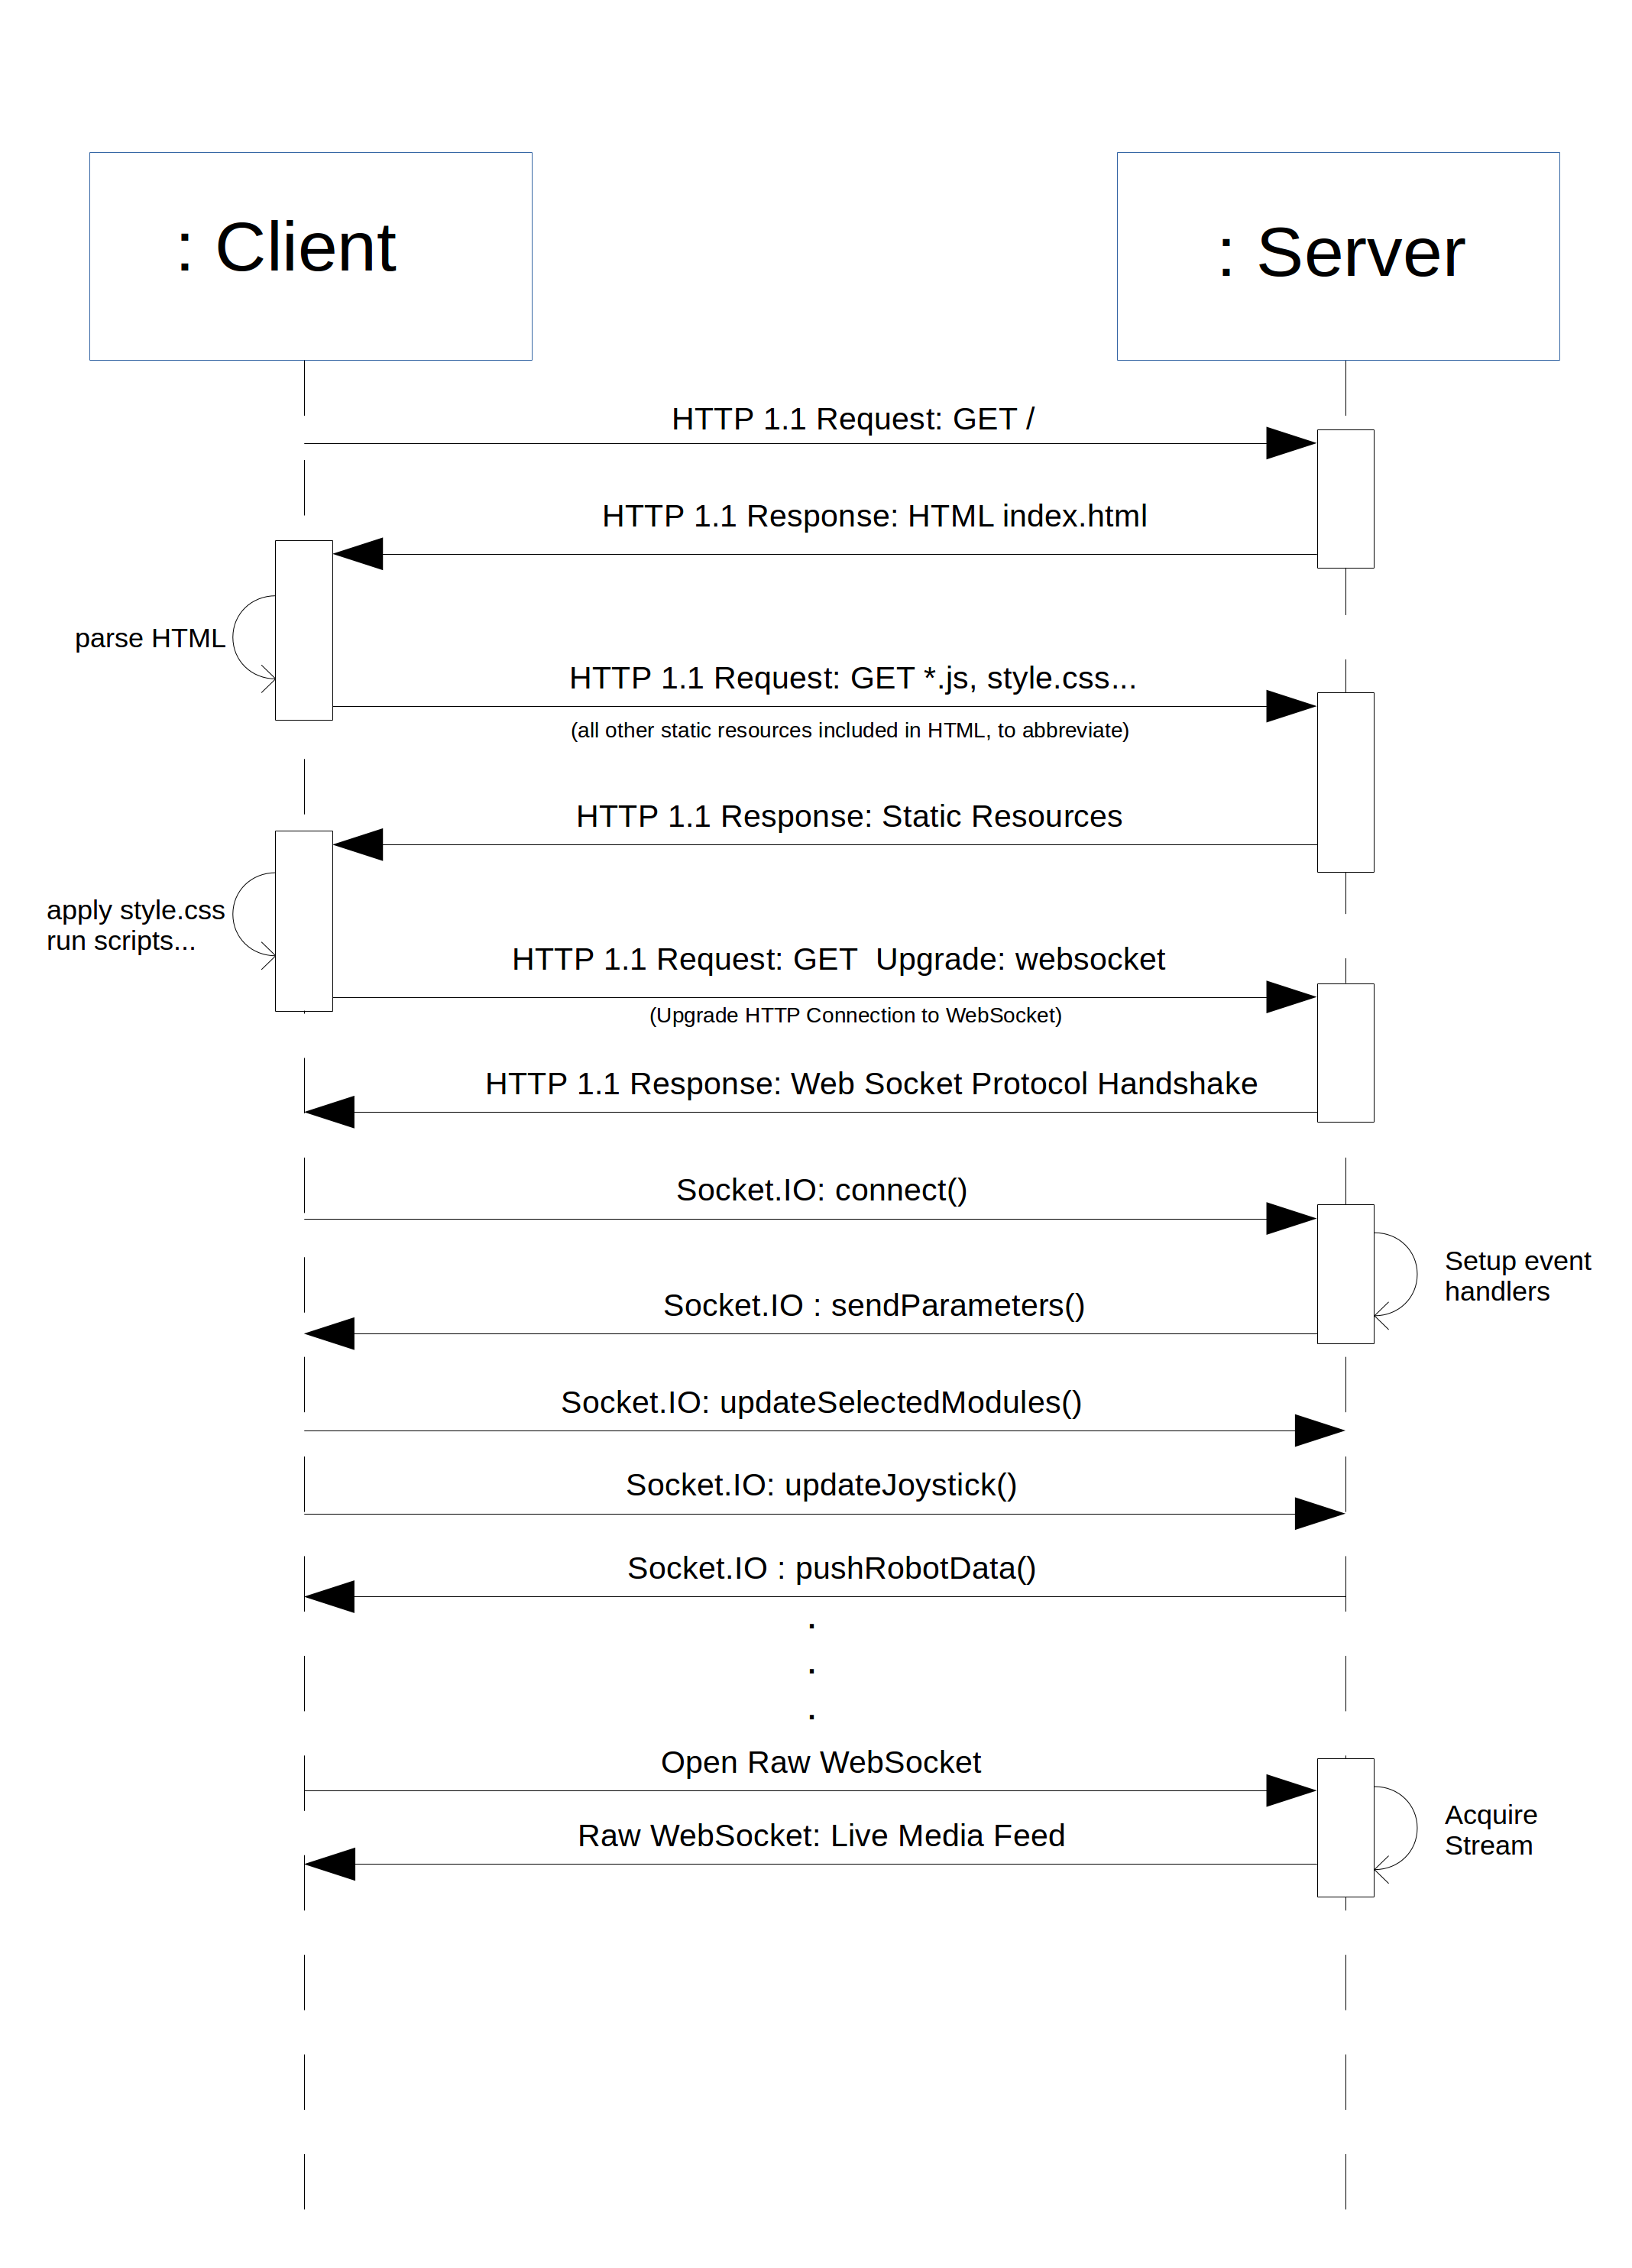
\includegraphics[width=\linewidth]{clientserverarch}
\caption{HRUI Client-Server Sequence Diagram \label{clientserverarch}}
\end{figure}
\section{Modular Front-end Architecture} \label{modularfrontendarchitecture}
This section describes the front-end (the part of the application that is ``front-facing'' from the user perspective, in other 
words, i.e. the Graphical User Interface or GUI) as a sub-system of HRUI. Previous sections \ref{mvcpattern} and 
\ref{clientserverpattern} described the application as a whole, from two different architectural perspectives. This section 
dissects one of the components of the application and describes it's internal functions, as it's considered complex enough to 
warrant further discussion.\\

The component described in depth here is presented in both previous perspectives: in the MVC pattern (section 
\ref{mvcpattern}) it's called the View; in the Client-Server pattern (section \ref{clientserverpattern}) it's the client. See 
those sections for a look at how this component interacts with the rest of the application from both perspectives.\\

The front-end (hereinafter also called client or view, without distinction) has a modular MVC architecture (the MVC paradigm 
is explained in section \ref{mvcpattern}). The MVC architecture stems from the fact the it's built using Google's AngularJS 
framework, which implements an MVC pattern. This technology is explained, along with it's MVC structure in section 
\ref{AngularJS}. The modular pattern is implemented to keep separate the distinct functions of the user interface, so that 
they can be used and re-used individually or in any grouping that is coherent with the particular application. Since HRUI 
aspires to be a universal interface which is also accessible from almost any web-capable hardware this is essential.\\

To be truly universal, HRUI has to be easily usable for virtually any robot, real or simulated. Robots are extremely varied in 
their functions, features, and ultimately in their inputs and outputs, which is what a user interface interacts with. Of 
course, each robot will have it's own API, but this challenge is already overcome by the back-end, by being totally 
interface-agnostic. What needs to be overcome by the front-end, is making user inputs easily adaptable to each robot, as well 
as being versatile in presenting the outputs. Some robots are mobile, some are not. Some have video cameras, some do not. Some 
require very specific sets of inputs, some are just generally controllable with a standard joy-pad controller. The modular 
nature of the front-end allows the user to tailor the interface on the fly to each application, seamlessly (also saving each 
configuration if required for future use, using the profile management module, explained in section \ref{profilemanagement}).
Being able to use any subset of the modules means that the interface adapts to each robot, and while very useful, no amount of 
modules could reasonably cover all the possible inputs and outputs that exist for robots, or generally any interactive system. 
That's why the custom input and custom data modules are provided, allowing the user to create new inputs and poll outputs 
dynamically, without any restriction on the nature of the data, and even better, without having to program a single line of 
code (of course, the programmer would have to gather the inputs on the back-end and store the outputs as well, but from a 
users perspective this is totally transparent). These modules are detailed in sections \ref{custominput} and \ref{customdata} 
respectively.\\

To be truly accessible, HRUI has to be usable on a wide range of hardware. This is already achieved, from a theoretical 
standpoint, by the nature of the View: it's an HTML5 web page, the de-facto standard for data communication worldwide. This 
also, by any reasonable measure, future-proofs the application, as HTML will likely continue to be relevant for many years to 
come, and with a history of backwards compatibility reigning supreme throughout the webs evolution (see section \ref{HTML} for 
more), it's not likely that HTML5 compliant pages, like HRUI's front-end will be deprecated any time soon. But the fact of the 
matter is: not all hardware that theoretically complies with HTML5 has the features required to run \textit{anything} that is 
HTML5 compliant. In other words, performance may vary on low-end hardware, especially if the web page is using a large amount 
of resources on the client-host. That's where modularity comes in: since it's not necessary to run every module to run one of 
them, even low-end hardware can use HRUI, albeit a diminished version of it. If the device cannot handle dual joysticks plus 
video and audio streaming plus device orientation, any of these modules, which might not be critical, can be completely 
disabled leaving the rest of the modules intact, and working. This is called \textbf{Graceful Degradation}, and is required 
for applications that target a wide array of devices. Graceful degradation is also relevant in the scenario where the browser 
that is used to access the web page complies with only some of the HTML5 standards, while some features remain unsupported. 
This is typical of mobile browsers, which vendors have a tendency to update less regularly than their desktop counterparts 
(victims of the same hardware fragmentation being described here as an issue for HRUI, and really any modern web application). 
If a feature in HRUI isn't supported by the browser, the rest of the features work regardless. This is the case with some of 
the more experimental features of HRUI like the gamepad module, voice commands module and live audio module (sections 
\ref{gamepad}, \ref{voicecommands}  and \ref{liveaudio} respectively).\\

Each module implements an MVC architecture itself by virtue of the AngularJS framework:
\begin{itemize}
	\item \textbf{Module View}: A div element in the HTML DOM (see section \ref{HTML}), that fully contains all the 
	presentation required for the module, isolating it from other module views both in the code and in the presentation. This 
	is emphasized visually with the box-shadow and borders (see section \ref{html5styling} on HTML5 styling) that surround 
	each module.
	\item \textbf{Module Controller}: Each module has a separate JavaScript .js file, in which it's controllers logic is held. 
	No module controller acts upon any other module controller, and they do not share information. The only caveat to this is 
	the main app controller, that manages the active modules, profile loading and saving and therefore must share information 
	with all modules. This does not break modularity, given that the main app controller does not hold any logic, merely 
	acting as an intermediary between controllers and back-end. In any case, all information is shared through a separate 
	entity, specifically designed by the AngularJS framework for this purpose: a service. see section \ref{AngularJS} for 
	more, although the complexity of the AngularJS framework is far outside of the scope of this report.	
	\item \textbf{Module Model}: The model is held in the AngularJS entity called the scope. The scope is associated with a 
	controller, and defines the data and methods that a particular controller can access. A controller cannot (it's most 
	certainly possible, but if the application adheres to the AngularJS framework and overall the MVC pattern like HRUI does, 
	it strictly shouldn't, and HRUI strictly does not) access, modify or in any way act upon data and methods outside of its 
	scope. In layman's terms as far as the controller is concerned, nothing exists outside of it's scope and it's logic deals 
	only with this model.
\end{itemize}

Apart from the benefits for the user, modularity has great benefits for future development, which will be briefly discussed in 
section \ref{futuredevelopment}.\\

The following sections briefly explain the functions of each module. Each section roughly includes a figure showing the module 
view in use, a brief explanation of what the module does, what APIs or externally developed software it may use if any, and if 
it's been used in the proof-of-concept integrations.  They're separated into three categories:
\begin{itemize}
	\item \textbf{Input Modules}: Used to give commands or more generally provide data to the application, and subsequently to 
	the robot.
		\begin{itemize}
			\item Joystick Module
			\item Gamepad Module
			\item Device Orientation Module
			\item Voice Commands Module
			\item Custom Input Module
		\end{itemize}
	\item \textbf{Output Modules}: Used to present data from the application model, typically from the robot.
		\begin{itemize}
			\item Data Monitor Module
			\item Live Video Module
			\item Live Audio Module
			\item Geolocation Module
			\item Custom Data Module
		\end{itemize}
	\item \textbf{Utility Modules}: Available for user convenience.
		\begin{itemize}
			\item Script Execution Module
			\item Profile Management Module
		\end{itemize}
\end{itemize}
\subsection{Input Modules}
\subsubsection{Joystick} \label{joystick}
\begin{figure}[H]
\centering
\captionsetup{justification=centering}
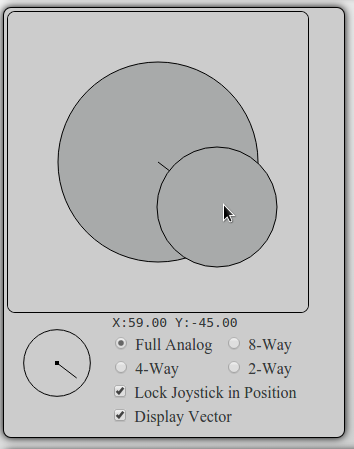
\includegraphics[width=0.5\linewidth]{joystick}
\caption{HRUI Joystick Input Module}
\end{figure}
The joystick module presents a virtual 2 dimensional joystick input that the user can manipulate either with the cursor or 
with touch, if the device is so enabled. It has four modes, that can be changed by the user at any given time, and provide 
bounds to the coordinates of the joystick, which may be appropriate for different applications (e.g. differential wheeled 
robots such as the Khepera III are generally controlled using ``tank'' controls, where the joystick only moves in the four 
cardinal directions):
\begin{itemize}
	\item Full Analog: the joystick can move freely inside its range.
	\item 8-Way: the joystick can only move on the Cartesian axes and on lines Y=X and Y=-X.
	\item 4-Way (Default): the joystick can only move on the Cartesian axes.
	\item 2-Way: The joystick can only move on line X=0.
\end{itemize}
Below the joystick itself is a visual representation of the vector created by the joystick, which can be toggled on (default) 
or off, as well as a dynamic print out of the current coordinates. The joystick can be toggled to stay in place or to return 
to the Cartesian origin (default) when released by the cursor or touch event.\\

The Joystick and the Vector are both HTML5 canvas elements (see section \ref{html5canvaselement}). The browser captures the 
mouse/touch events (down, move, up) and gives the controller a coordinate of where the cursor is. The canvas element is then 
redrawn with the circle that represents the joystick (and the line that represents the vector) centered around the coordinate. 
This is done at 60 FPS (frames per second), giving the illusion of animation to the user. The coordinates are also sent to the 
back-end at this refresh rate (approximately 16 ms), with the currently enabled mode. The coordinate print out is only updated 
roughly every 240ms for efficiency, since the resolution required for actual use of the inputs is not necessary for the users 
visual feedback.\\

This module was the first input to be developed for the application. It was made initially for the V-REP virtual Khepera III 
proof-of-concept integration, and was also used to control the real Khepera III's movement in 4-way mode. It has been used in 
conjunction with the device orientation module for the latest integration (not presented in this report for time constraints) 
with the Parrot Rolling Spider drone. The joystick controls the movement of the drone on the horizontal plane.
\subsubsection{Gamepad} \label{gamepad}
\begin{figure}[H]
\centering
\captionsetup{justification=centering}
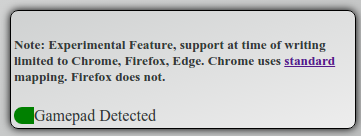
\includegraphics[width=0.5\linewidth]{gamepad}
\caption{HRUI Gamepad Input Module}
\end{figure}
This module takes the inputs from any generic gamepad controller that is connected to the client-host and detected by the 
browser and sends them to the back-end for use. It uses the HTML5 Gamepad API which at time of development is still in an 
experimental phase, and hasn't been implemented by all browsers. More disruptively, the browsers that have implemented it, 
have used different key-mapping for the gamepad. This should be resolved in the near future, given that the specification 
actually presents the recommended layout\cite{w3cgamepad15}, but in the mean time, care should be taken when designing a 
controller to somehow account for these differences (normally, using a short combination of keys to work out what layout is 
being used). The only web browsers that have technically implemented the API at time of writing, in their latest versions are 
Google Chrome (and most Webkit based browsers, though not all of them), Mozilla Firefox and Microsoft Edge. The availability 
of the API can be determined using tools like caniuse.com\cite{caniusegamepad15}. Another issue is that some browsers require 
a button to be pressed for initial detection, and others require the web page to be visible on screen for inputs to be 
registered.\\

Aside from these growing pains, this module provides almost infinite extensibility to the application. Any hardware device 
that can be recognized by the client-host browser can be used as an input, and if it's really necessary, there are tools that 
can map any input to a computer to a ``virtual gamepad'', that would then be recognized by the browser and therefore usable 
through HRUI.\\

This module has been used to control all three proof-of-concept robots, but is specially required in the case of the Crazyflie 
2, as it has no stability or altitude control (lacks the instrumentation necessary), and it's light weight makes very 
sensitive to inputs (but makes it blazing fast as well). The gamepad can be used outside local networks, on cellular internet 
even, and the responsiveness does not suffer one bit.\\

The module has been tested by the developer in the following configurations successfully (note: this is not an all-inclusive 
list, other configurations probably work as well):\\
\begin{itemize}
	\item Wired Xbox 360 Controller (USB): 
		\begin{itemize}
			\item Wired to a laptop computer, using Google Chrome, Mozilla Firefox (Linux and Windows) and Microsoft Edge 
			(Windows 10).
			\item Wired through a USB OTG (on-the-go) adapter to an android smartphone (Sony Xperia Z3, Android 5.1) running 
			Google Chrome (presented mapping issues with right analog stick), Mozilla Firefox and Opera Mobile.
		\end{itemize}
	\item Wireless PS4 Dualshock 4 Controller (Bluetooth):
		\begin{itemize}
			\item Paired through bluetooth to a laptop computer , using Google Chrome, Mozilla Firefox (Linux and Windows).
			\item Paired through bluetooth to an android smartphone (Sony Xperia Z3, Android 5.1) running Google Chrome 
			(presented mapping issues with right analog stick), Mozilla Firefox and Opera Mobile.
		\end{itemize}
\end{itemize}
\subsubsection{Device Orientation} \label{deviceorientation}
\begin{figure}[H]
\centering
\captionsetup{justification=centering}
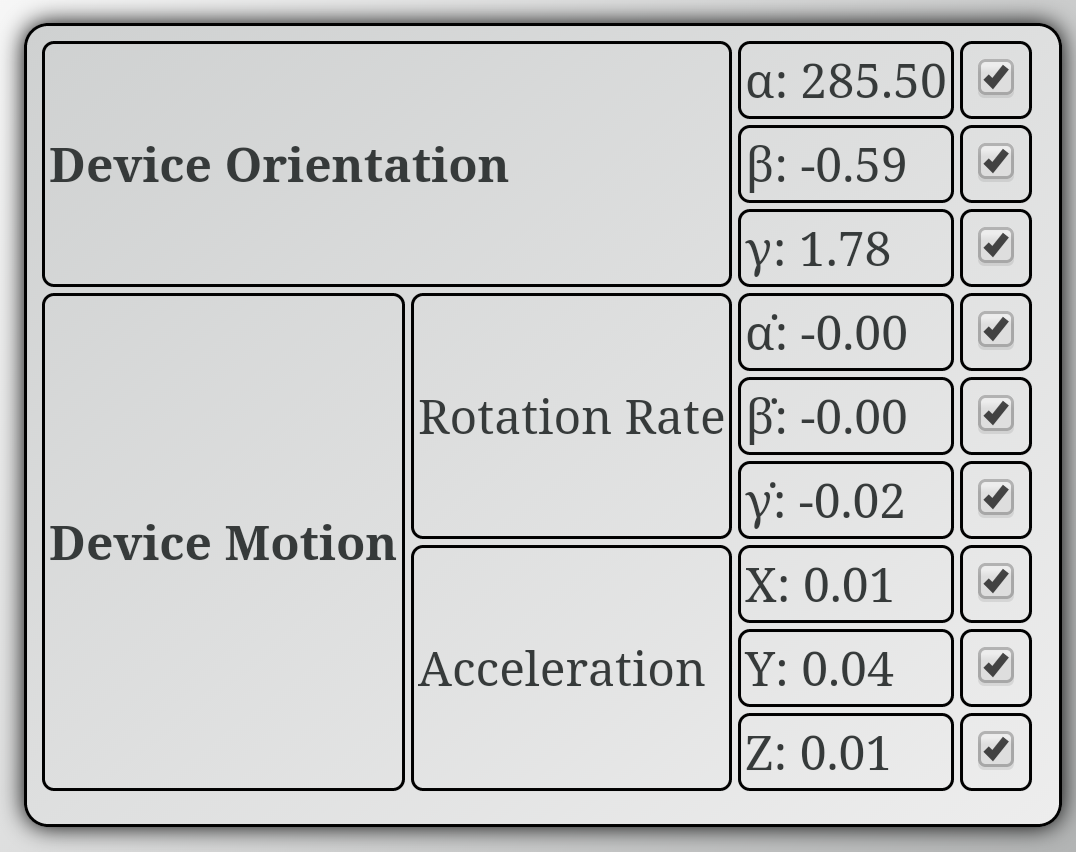
\includegraphics[width=0.5\linewidth]{deviceorientation}
\caption{HRUI Device Orientation Input Module}
\end{figure}
Captures the client-host device orientation and motion data if available. It uses the HTML5 Device Orientation and Device 
Motion APIs, which can be implemented independently. The interface checks for the availability of the APIs and subsequently if 
the device has the hardware required for the measurements. If any, the captured values are sent to the back-end and can be 
used as inputs.  The values are updated at 60 FPS (roughly every 16ms), but the presented values are updated every 240ms, for 
efficiency. The module allows ``spoofing'' certain values, by disabling further updates of selected angles or rotation rates, 
simply using a check-box. This enables the user, for example, to make the controller believe the device is totally horizontal 
by laying the device on a flat surface, unchecking the beta angle check-box, and then moving the device for easier use.\\

It has been used in conjunction with the joystick module for the latest integration (not presented in this report for time 
constraints) with the Parrot Rolling Spider drone. The beta angle (the vertical inclination of the device, i.e. when holding a 
smartphone, the angle formed by the plane defined by the screen and horizontal plane) controls the vertical movement of the 
drone. It was used in a more crude control scheme to ramp up the thrust of the motors for the Crazyflie 2. Given that this 
drone doesn't have altitude control (the Rolling Spider does, as it has an ultrasonic sensor on it's underside), the same 
control isn't feasible for it.
\subsubsection{Voice Commands} \label{voicecommands}
\begin{figure}[H]
\centering
\captionsetup{justification=centering}
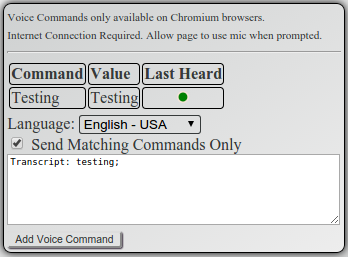
\includegraphics[width=0.5\linewidth]{html5_voice}
\caption{HRUI Voice Commands Input Module}
\end{figure}
Used to input voice commands from the client device. The steps involved in this process are as follows:
\begin{enumerate}
	\item On module activation, requests access to the client device microphone if available. The user must grant access 
	manually each time the module is activated or the input language is modified. This is a limitation of the HTTP protocol, 
	for security reasons. If the application was ported to the HTTPS protocol, it would only be necessary to grant access once.
	\item Once access to the microphone has been granted, captures speech input continuously. If sound level is too low, the 
	capture will stop and access to microphone will have to be granted again.
	\item Using an Internet connection (required), sends the captured speech for recognition using the webkit Speech API.
	\item Receives the result, and compares it to the set of commands inputted by the user.
	\item If the command matches the result of speech recognition, signals the matched command to the user and sends the 
	command and it's assigned value to the back-end, for use.
\end{enumerate}
This feature is still very much experimental, given that the HTML5 Speech API is relatively new to the standard (proposed in 
2012), and as of the writing of this report has only been implemented by Chromium browsers\cite{caniusespeech15}. However, it 
works perfectly if used with the latest Google Chrome, both on mobile (tested on Android 5.1 and 4.4.4) and desktop versions. 
The ability to create commands on the fly and parse the speech result, all on the client side, reduces greatly the work for 
the programmer on the back-end: the only required processing is polling the model (mongodb database) for the required command. 
Adding the ability to attach a value different than the command itself makes it even simpler: if the user wants several 
commands to correspond with the same input, all that's necessary is to assign the same value to them, and the programmer only 
needs to poll this value, without having to process what command generated it. This results in a very versatile and accurate 
input, although the recognition speed is still lacking, as it's done remotely, so recognition is delayed by a second or so. 
this is not a fault of the application, it's just simply the state of the art of web speech recognition.\\

The module uses the external JavaScript library ``annyang!'' by Tal Ater\cite{annyang15}, used under the MIT License (see 
section \ref{opensourcemovement} for more on open source licensing). If the browser doesn't support the HTML5 Speech API, the 
module offers an alternative: recording 5 seconds of audio that is sent to the back-end as a .wav file, for external 
processing. This alternative is experimental and does not work on all browsers. The alternative uses the external JavaScript 
library RecordRTC\cite{recordrtc15}, used also under the MIT License. In any case, failure of the module to function in no way 
inhibits the application, by virtue of it's modularity, explained in section \ref{modularfrontendarchitecture}\\

The module supports the following languages, although with small changes, almost any language can be added:\\

English, Spanish, Italian, French, German, Mandarin, Japanese, Arabic and Hindi;\\

This input was used successfully as an ``emergency'' landing input when flying both the Crazyflie 2 and the last integration 
(not documented fully for time constraints and due to being very similar to other integrations), the Parrot Rolling Spider. On 
detection of the word ``stop'', the controller would stop executing the orders received from the gamepad or joystick, and 
progressively wind down the thrust of the propellers, or in the case of the Rolling Spider, reduce altitude until ground was 
detected.
\subsubsection{Custom Input} \label{custominput}
\begin{figure}[H]
\centering
\captionsetup{justification=centering}
\subfloat{\raisebox{65px}{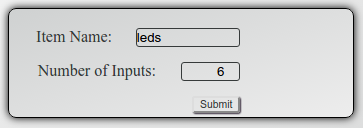
\includegraphics[width=0.33\linewidth]{custominput1}}}
\subfloat{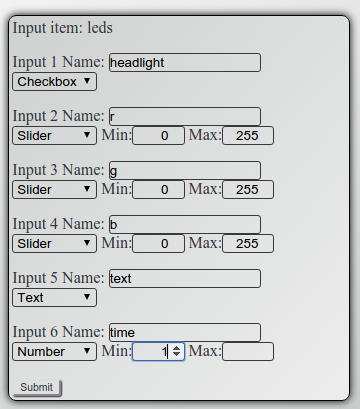
\includegraphics[width=0.33\linewidth]{custominput2}}
\subfloat{\raisebox{20px}{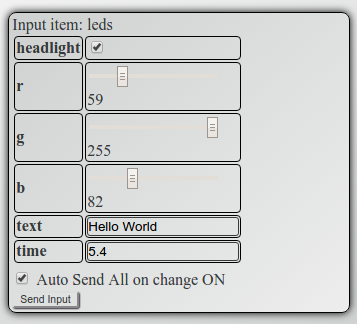
\includegraphics[width=0.33\linewidth]{custominput3}}}
\caption{HRUI Custom Input Module}
\end{figure}
This module allows the user to create any input that may not be covered with other modules, simply by inputing the item name, 
the number of inputs and the type of each input. The input can then be recovered in the back-end as simply as any other input 
module, by retrieving the item name from the database and using the data accordingly. This grants almost infinite versatility 
to the application, allowing up to 50 different inputs (the number is arbitrary and could be extended to any number by 
changing one value in the HTML) to be created (and saved in a profile for easy reuse through the profile management module, 
see section \ref{profilemanagement}) at any point during the execution of the application. The programmer if he so wished, 
could easily create a completely custom interface with this module, by providing the controller that uses the inputs and 
providing the user with instructions on how they work, never having to use any of the other modules. The process of generating 
the inputs is as follows (see the image at the start of this section from left to right for reference):
\begin{enumerate}
	\item On module activation, the module requests the custom input item name, and the number of inputs it holds.
	\item Once the input item and number of inputs is given, the module presents a form with an input name and type for each 
	of the requested inputs. The types offered are:
		\begin{itemize}
			\item Text: A string of characters.
			\item Number: A number, with dot formatting for decimals. A minimum and maximum value can be provided (both 
			independently optional).
			\item Slider: A numeric value that can be controlled using a virtual sliding control. A minimum and maximum value 
			must be provided.
			\item Check-box: two-state control. Can be checked or unchecked.
		\end{itemize}
	Please note that these four types cover all the basic "primitive" data types, thus giving a simple interface for any 
	reasonable unitary input: the number can be an integer or decimal; the string covers characters and the check-box covers 
	boolean values (true or false).
	\item Once the previous form is submitted, the controls are presented to the user in a table. The user can then manipulate 
	the inputs, sending them manually to the back-end using a button, or allowing automatic updates to occur when values are 
	changed (default). In the back-end, the programmer can simply pull the item from the database and get all the inputs 
	organized by the name given by the user.
\end{enumerate}
It's important to note that at no point in this process has the page been refreshed or has the source HTML been modified. This 
might seem trivial but this would be impossible only a few years ago, given that the new HTML that's being generated 
dynamically (notice: the application has no knowledge of the names, number and types given by the user until inputted) 
couldn't be ``recompiled'' without re-parsing the HTML, that would have to be served statically from the server (this would 
usually entail a CGI script feeding the HTML into the browser). This is possible due to the AngularJS framework, that not only 
can recompile the HTML, but can then data-bind the values in that HTML to a dynamically generated JavaScript object (notice: 
the object cannot be defined at the initial run-time, only after the user declares it) that is sent in real-time through 
web-sockets to the back-end. See section \ref{AngularJS} for more on the AngularJS Framework.\\

This module has been used successfully in the Crazyflie 2 integration. The Crazyflie 2 has an extension board of LEDs (Light 
Emitting Diodes) positioned in a ring formation under the drone. This extension board also has a headlight pointing forward. 
The image at the beginning of this section shows the setup required for the control of this extension board (the last two text 
and number inputs are not used, but are added in the image for reference in the previous explanation). With this setup and the 
back-end code presented in figure \ref{ledcode}, it's possible to dynamically change the colors of the LEDs by changing the 
RGB (Red Green Blue) values (sliders between 0 and 255) to match the desired color, as well as turn the headlight on and off 
(check-box: checked = true, unchecked = false). As is evident, the effort required on both the users part (the modules' state 
can be saved to a profile so it wouldn't even be necessary to do anything other than load the profile) and the programmers' 
part (12 lines of self-explanatory code, that goes up to 20 or so when adding all required fail-safes) is minimal.
\begin{figure}[H]
\captionsetup{justification=centering}
\RecustomVerbatimEnvironment{Verbatim}{BVerbatim}{}
\begin{minted}[fontsize=\footnotesize]{python}
def ledcontrol():
	headlight = -1
	rgb = [0, 0, 0]
	while True:
		newLeds = data.find_one({"item": "leds"})
		headlight = newLeds['headlight']
		rgb[0] = newLeds['r']
		rgb[1] = newLeds['g']
		rgb[2] = newLeds['b']                
		crazyflie.param.set_value("ring.headlightEnable", str(headlight))                
		crazyflie.param.set_value("ring.solidRed", str(rgb[0]))                
		crazyflie.param.set_value("ring.solidGreen", str(rgb[1]))                
		crazyflie.param.set_value("ring.solidBlue", str(rgb[2]))
\end{minted}
\caption{HRUI Crazyflie Integration: LED Expansion Board Control code (Abridged)\label{ledcode}}
\end{figure}
\subsection{Output Modules}
\subsubsection{Data Monitor} \label{datamonitor}
\begin{figure}[H]
\centering
\captionsetup{justification=centering}
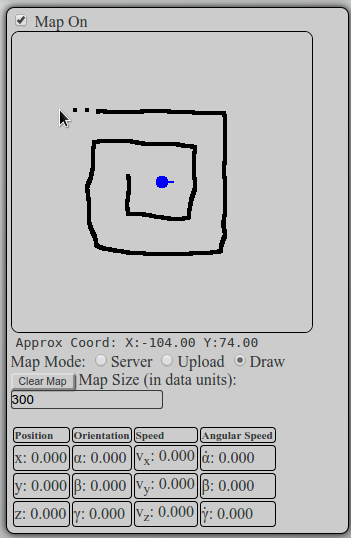
\includegraphics[width=0.5\linewidth]{html5_map}
\caption{HRUI Data Monitor Output Module}
\end{figure}
This module provides the basic data outputs received from the robot, as well as a multi-mode map. The data is presented in a 
table format and includes:
\begin{itemize}
	\item Position: $X, Y, Z$ coordinates.
	\item Orientation: Euler Angles $\alpha, \beta, \gamma$.
	\item Speed: $V_x$, $V_y$, $V_z$.
	\item Angular Speed: $\dot{\alpha}, \dot{\beta}, \dot{\gamma}$
\end{itemize}
It's important to point out this isn't meant to cover any and all possible outputs from a robot, as that would be impossible. 
This only covers basic positioning, orientation and speed, as these values pertain to the location and mapping of the robot 
and it's surroundings. Any other outputs (as well as inputs, if so desired) can be monitored easily using the custom data 
module, explained in section \ref{customdata}. No units are provided for the data, as the scale would hardly be universal.\\

The map is a square, 300x300px HTML5 canvas element (see section \ref{html5canvaselement}), initially representing the robot 
on a 2d plane as a blue dot, with a vector to show it's orientation. The scale of the map can be set by the user dynamically, 
and is to be coherent with the unit for the data provided, given that the blue dot representing the robot will move 
dynamically inside and outside the bounds of the map when the position and orientation values received are updated. This can 
be deactivated in Server mode, making the blue dot stay in the center facing up, to support the map feed being relative to the 
position of the robot. The map can function in three distinct modes:
\begin{itemize}
	\item \textbf{Server Mode}: The map is pulled from the server approx. every 200ms. The map is held in the model of the 
	application as a 300x300 binary matrix, composed only of ones and zeros, with one representing an obstacle, and zero 
	representing free space. This matrix can be manipulated by a controller freely, and the result will be displayed in the 
	front-end with white representing free space (zero) and black representing obstacles (one). The manner in which the binary 
	matrix is generated isn't part of the application, but it could be generated using SLAM (Simultaneous Localization and 
	Mapping) techniques, or in whatever pertinent way, very easily.
	\item \textbf{Upload Mode}: The user uploads to the server, through a file selection menu, a JPEG or PNG image that is set 
	as the map. This can be useful for preprogrammed circuits or maze experiments.
	\item \textbf{Draw Mode}: The user can draw obstacles on the map directly by using the cursor or touch, if the client-host 
	is so enabled. This black and white canvas is then stored in the model in real-time in the same place and manner as the 
	binary matrix explained in Server Mode. The approximate coordinates (in data units) of the cursor are presented to the 
	user for convenience. This mode has many possibilities: since the binary matrix is accessible to the robot controller, the 
	obstacles generated by drawing can be used to modify the robots behavior, making it stop, or navigate around the obstacle, 
	or whatever is relevant to the robot application or experiment. Another application could first let the user enter Draw 
	Mode, make a drawing of the obstacles, then enter Server Mode, and generate on top of this drawing the actual readings 
	from the robots instrumentation, to see how well it matches up. The possibilities are almost endless, since the model is 
	so easily modifiable.
\end{itemize}
This module, in it's simplest form, only with the table of positioning and orientation, was the second to be implemented in 
the application, after the joystick was implemented to get the data from the V-REP virtual Khepera III and present it on the 
page.\\

The map was used in upload mode (without a background) with the V-REP virtual Khepera III, with the scale matched to the 
virtual environment in the simulator. The blue dot changed orientation and position according to the data fed by the 
simulator, granting a completely independent 2D representation of the simulation, as well as the input control provided by the 
joystick. It was also tested using the physical Khepera III, although getting coordinates was much harder, given that the 
output from the robot is the encoder position of the wheels. Mapping was still possible, given that tank controls can be 
modeled with some effort: when turning, all coordinates remain unchanged and the euler beta angle has to be changed 
accordingly; when going forward or backward, using the beta angle that remains unchanged, the x and y coordinates can be 
extracted; This provided the x and y coordinates for the map, but accuracy rapidly decreased with extended use, as the encoder 
values cannot be totally accurate and normal movement jolts not registered by the encoders made the model unreliable. In any 
case, this is out of the scope of the application: representation of the data was correct; acquisition of said data is part of 
a whole different problem, that pertains to the robot programmer or researcher.\\

In server mode and draw mode, the map was tested and works as explained and expected. No actual application was developed for 
these modes, as SLAM falls outside the scope of this project, being almost a field of study in itself. The tests were made 
using a python script that generates random values for the binary matrix, which expectedly present a ``white noise'' dynamic 
pattern (similar to that of old analog television static) when viewed in the module. Drawing tests were made by drawing 
certain sections and inspecting the matrix to see if the sections were registered as ones.\\

This module uses "node-pngjs"\cite{nodepngjs12} and "busboy"\cite{busboy13} under the MIT License.
\begin{figure}[H]
\centering
\captionsetup{justification=centering}
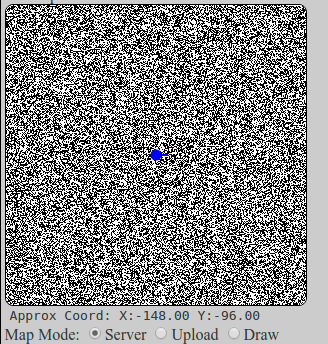
\includegraphics[width=0.3\linewidth]{servermode}
\caption{HRUI Data Monitor: Server Mode random binary matrix test}
\end{figure}
\begin{figure}[H]
\captionsetup{justification=centering}
\RecustomVerbatimEnvironment{Verbatim}{BVerbatim}{}
\begin{minted}[fontsize=\footnotesize]{python}
n = 300
M = np.zeros((n,n));
while True:
	for j in xrange(0,n):
		for i in xrange(0,n):
			if (np.random.rand(1)[0] >= 0.5):
				M[i][j] = 0
			else:
				M[i][j] = 1
	Mj = json.dumps(M.tolist())
	data.update({"item": "mapData"}, {"set": { "map": Mj, "_id": 5 } }, True)
\end{minted}
\caption{HRUI Binary Matrix generation example (random matrix) (Abridged)}
\end{figure}
\subsubsection{Live Video} \label{livevideo}
\begin{figure}[H]
\centering
\captionsetup{justification=centering}
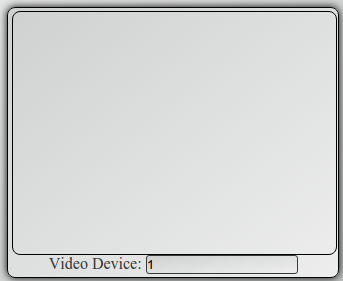
\includegraphics[width=0.5\linewidth]{video}
\caption{HRUI Live Video Output Module}
\end{figure}
Outputs a live video feed captured in the back-end. Playback is fully compatible with any HTML5 compliant browser, given that 
the video is decoded natively using JavaScript, instead of relying on any external software that would rely on the browser 
supporting that particular format. The decoded video is presented using an HTML5 canvas element (see section 
\ref{html5canvaselement}), where each frame is output and refreshed at 60 FPS, giving the illusion of video. The video is 
received as a bit stream delivered through WebSockets. See section \ref{clientserverpattern} for more on the client-server 
communications, and section \ref{html5websockets} on HTML5 WebSockets. The JavaScript MPEG Layer 1 video decoder is external software called ``jsmpeg''\cite{jsmpeg15}, integrated into the project under the MIT License.\\

Live streaming is only available if the application is deployed on a Linux platform. This is because external software is 
required for stream acquisition and because of the way this stream acquisition is handled at the Operating System level. Linux 
presents an interface for external devices called device files. These files are stored in the path ``/dev'', and appear on 
external device detection. Video devices appear as ``videoX'' files, where X is an integer that identifies the device if more 
than one are present. Upon module activation, HRUI makes a call to run the previously mentioned external software, called 
avconv\cite{avconv15}. FFMpeg can be optionally used as well if preferred by the server administrator. This external program 
uses the device file to start acquiring the bit stream, and HRUI relays the stream to the user. If more than one video device 
is present, the user can change from one to the other dynamically using the input box in the module. This can be useful if, 
for example, the robot has a front-facing and rear-facing camera. Using the device file system has the advantage of 
simplifying data acquisition, as it's very simple to generate the file for other video sources (for example, tweaking the 
arguments of the avconv call, it's possible to stream the VGA output of the server as video).\\

Live streaming video has been tested with the Khepera III integration, using the Raspberry Pi 2 as a server. This was tested 
even over cellular Internet and lag is very low. See figure \ref{kheperaiiidemo} and the associated video link for a 
rudimentary demo. The mentioned method of streaming the screen output of the server-host was tested in the V-REP virtual 
Khepera III integration, to stream the simulation window.
\subsubsection{Live Audio} \label{liveaudio}
\begin{figure}[H]
\centering
\captionsetup{justification=centering}
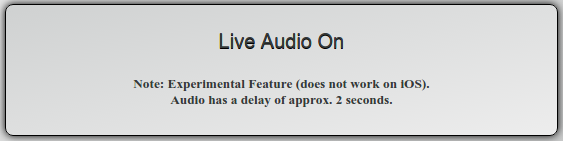
\includegraphics[width=0.5\linewidth]{audio}
\caption{HRUI Live Audio Output Module}
\end{figure}
Outputs a live audio feed captured in the back-end. This module is experimental and does not work on some devices, 
particularly iOS based devices. This is not because it uses any external software that isn't native, and the reasons 
unfortunately haven't been documented in the project, although effort was put in to find the issue. The stream has 
significant lag, that hovers around 2 seconds. This also hasn't been improved, although at the beginning of development, the 
lag was significantly higher, and through code optimization was reduced. It doesn't work consistently across audio capturing 
devices, depending on the number of channels provided by the hardware. This can be tweaked in the back-end.\\

The module uses the external decoder framework aurora.js\cite{aurora15} for the pure JavaScript MP3 decoder, and an adapter 
to accept WebSocket input, aurora-websocket\cite{auroraws15}. Both are used under the MIT License. Again, both are completely 
native solutions that require no compatibility on the browser side, so this is not the source of the issues mentioned.\\

Live streaming audio has been tested with the Khepera III integration, using the Raspberry Pi 2 as a server. This was tested 
even over cellular Internet and lag remained constant, at 2 seconds approx.
\subsubsection{Geolocation} \label{geolocation}
\begin{figure}[H]
\centering
\captionsetup{justification=centering}
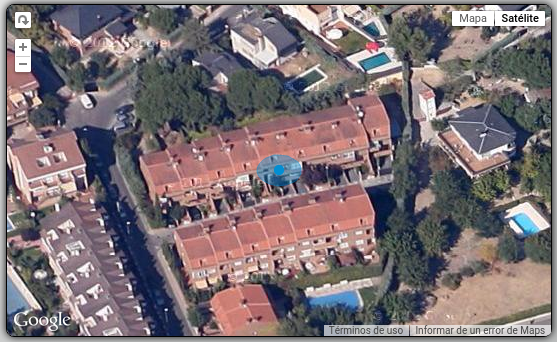
\includegraphics[width=0.5\linewidth]{geolocation}
\caption{HRUI Geolocation Output Module}
\end{figure}
Presents a map that tracks the latitude and longitude of the robot. The map is generated using the Google Maps API
\cite{googlemaps15}. Once the module is active, the latitude and longitude of the robot is retrieved periodically from the 
model in the back-end as well as the accuracy in meters of the measurement. This is sent to the front-end where a map is 
shown around a blue dot that represents the robot, and a translucent blue circle that represents the accuracy of the 
location, and has the diameter of the accuracy provided.\\

The Google Maps API is used in it's HTML5 compliant form, that uses an HTML5 canvas element (see section 
\ref{html5canvaselement}) to output the map. The user can change the zoom, map type and visual angle, as well as momentarily 
pan away from the robot, though on each update, the map is re-centered on the robot.\\

Since none of the used robots has geolocation capabilities, this module has not been tested in any of the integrations. 
However it has been tested using a simple test script that changes the value of the robot latitude periodically, so the map 
can be seen to pan correctly.\\
\begin{figure}[H]
\captionsetup{justification=centering}
\RecustomVerbatimEnvironment{Verbatim}{BVerbatim}{}
\begin{minted}[fontsize=\footnotesize]{python}
while True:
	geolocation = data.find_one({"_id": 2})
	latitude = float(geolocation['latitude'])
	data.update({"item": "robotGeolocation"}, 
				{"set":{"latitude": latitude+0.0000001}})

\end{minted}
\caption{HRUI Geolocation generation example script (Abridged)}
\end{figure}
As an easter egg, the initial location of the map before the first update from the server is the authors location for the 
majority of the project development.
\subsubsection{Custom Data} \label{customdata}
\begin{figure}[H]
\centering
\captionsetup{justification=centering}
\subfloat{\raisebox{20px}{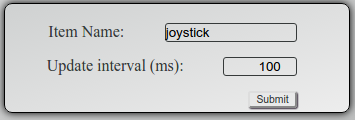
\includegraphics[width=0.5\linewidth]{customdata1}}}
\subfloat{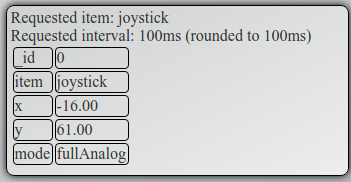
\includegraphics[width=0.5\linewidth]{customdata2}}
\caption{HRUI Custom Data Output Module}
\end{figure}
This module allows the user to poll any item from the application model, at a specified interval. The process is as simple as 
inputting the desired item and the desired update interval. The module generates a table with the data organized recursively. 
This means that not only the top level keys in the item are represented. If the key is an object itself, the child properties 
of the object are presented as well, differentiated by using HTML header table elements, that emphasize each object name 
visually. This provides almost infinite extensibility to the output modules of HRUI, since any data that can be stored in the 
model can be presented to the user simply by exposing the name of the item. Furthermore, this also includes anything that is 
in the model, therefore inputs can be monitored as well. This has many possibilities, such as an administrator monitoring the 
use of the HRUI application by others, by polling, for example, the joystick item as is presented in the figure at the 
beginning of this section.\\

It's important to note that at no point in this process has the page been refreshed or has the source HTML been modified. 
This might seem trivial but this would be impossible only a few years ago, given that the new HTML that's being generated 
dynamically (notice: the application has no knowledge of the items required by the user, or the update interval until 
inputted) couldn't be ``recompiled'' without re-parsing the HTML, that would have to be served statically from the server 
(this would usually entail a CGI script feeding the HTML into the browser). This is possible due to the AngularJS framework, 
that not only can recompile the HTML, but can then data-bind the values in that HTML to a dynamically generated JavaScript 
object (notice: the object cannot be defined at the initial run-time, only after the user requests it) that is received in 
real-time through web-sockets from the back-end. See section \ref{AngularJS} for more on the AngularJS Framework.
\subsection{Utility Modules}
\subsubsection{Script Execution} \label{scriptexecution}
\begin{figure}[H]
\centering
\captionsetup{justification=centering}
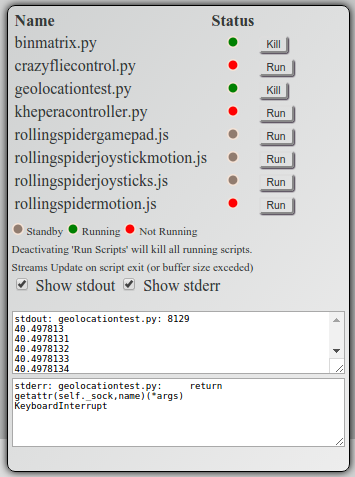
\includegraphics[width=0.5\linewidth]{scriptexecution}
\caption{HRUI Script Execution Utility Module}
\end{figure}
This utility module is made available for the convenience of users who are also server administrators, robot programmers or 
researchers. It allows the user to execute and kill any Python or Node.js script that is made available in the server in the 
folder ``userscripts''. It also redirects the standard output and standard error channels to the user (can be toggled on or 
off individually), as well as showing the current state of the script with a color code:
\begin{itemize}
	\item Grey: The script has not been executed. Note this only includes executions from this instance of the client. If the 
	script is run locally on the server or other clients run the script, this will not change the state of the indicator.
	\item Green: The script is currently in execution after being run from this instance of the client.
	\item Red: The script is currently not running after being run from this instance of the client. This can be because the 
	script has finished, exited because of an error, or because the user killed it using the kill button provided.
\end{itemize}
This makes testing the HRUI front-end and the robot controllers much easier and faster. The use of this module was thought of 
during the development, for the developers convenience. This tool should also supply a solution for any additional needs to 
configure the server for a specific application of HRUI. Initially this module was going to be a full on SSH client that 
allowed the user to open a remote terminal on the server, granting full access. This of course is a security issue, and would 
have to be developed with a lot of care, as well as being well beyond the scope of the project. This solution is a 
compromise, granting the functionality required while remaining secure, since the user cannot upload the scripts that are 
being executed. The scripts have to previously been placed in the folder manually, with direct access to the server. If 
malicious software is planted manually in the server, the security of the server is already compromised regardless of being 
remotely executed through HRUI.\\

This was used thoroughly in all of the integrations, as it allows the execution of the robot controller remotely, before 
using 
the actual inputs and outputs provided by the interface. The image shows many of the integration controllers, as well as the 
undocumented Parrot Rolling Spider integration and the binary matrix and geolocation test scripts explained in sections 
\ref{datamonitor} and \ref{geolocation} respectively.\\

Note that it's not obligatory to use this module to run the controllers, as the application works independently from the 
actual robot controllers as explained in section \ref{mvcpattern}, nor are the scripts that are in the userscripts folder 
necessarily robot controllers. This is a utility module and is therefore to be used as a tool for any purpose necessary.
\subsubsection{Profile Management} \label{profilemanagement}
\begin{figure}[H]
\centering
\captionsetup{justification=centering}
\subfloat{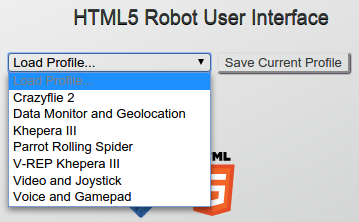
\includegraphics[width=0.5\linewidth]{profilemanagement1}}
\subfloat{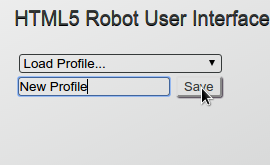
\includegraphics[width=0.5\linewidth]{profilemanagement2}}
\caption{HRUI Profile Management Utility Module}
\end{figure}
This module is used to save the current state of the front-end to be retrieved later, at the convenience of the user. This is 
particularly useful when using the custom input module (see section \ref{custominput}) with a large amount of inputs, given 
that every input has to be named and it's type selected manually by the user. This is fine if there's one or two inputs, but 
if there's 10 or 20, inputting the names manually on each use would be cumbersome. This also allows the user to setup 
particular module combinations for each of the robots that have been integrated with the application, given that every robot 
will have a different set of features, not all modules will be necessary or compatible with all robots. Another application is
for the programmer to set up a particular set of custom inputs, and the modules that the designed robot controller uses, so 
the user doesn't have to setup the interface, if the user doesn't happen to know anything about the controller. There are 
many possibilities, as the profiles are very easy to save and retrieve.\\

The module registers all of the active modules, and all of the settings inside of each of them, and stores these values in 
the application model, in the item named ``profiles''. The user can give each profile saved a name, for easy reference when 
loading the module subsequently.\\

This is done, as briefly mentioned in section \ref{modularfrontendarchitecture} by each of the modules sharing their model 
(their scope variables) with a parent controller, the main app controller. The main app controller gathers all of the model 
data (by generating a module-wide event), creates an object with all of it, and sends it to the back-end where it's stored in 
the model. To prevent breaking the MVC architecture by controllers manipulating other controllers model, this is done through 
an intermediary object specifically designed to share data between controllers: a service. A service is a singleton object 
(in OOP, an object of which there can only be one instance throughout runtime) that merely holds properties that are meant to 
be manipulated by controllers, or holds methods that can be used by controllers to avoid repeating code. All of this is part 
of the AngularJS Framework, that allows, as stated in sections \ref{custominput} and \ref{customdata}, to generate HTML, 
particularly a modification of the DOM in this case, without having to regenerate the actual HTML structure. See section 
\ref{AngularJS} for more on the AngularJS Framework.